\part{Real Analysis}
\chapter{Number Systems}
\section{Natural Numbers $\NN$}
\subsection{Construction}
In Peano's development, it is assumed that there is a set $\NN$ (the natural numbers) of undefined objects with a distinguished element $1$ such that
\begin{enumerate}[label=(\roman*)]
\item $1$ is a natural number; that is $1\in\NN$;
\item every $n\in\NN$ has a successor $S(n)\in\NN$;
\item for every $n$, $S(n)\neq1$ (there is no number with 1 as successor)
\item if $S(n)=S(m)$, then $n=m$;
\item if $A$ is a set of natural numbers such that $1\in A$ and
\[n\in A\implies S(n)\in A,\]
then $A$ contains all natural numbers.
\end{enumerate}

\subsection{Properties}
\begin{theorem}[Archimedean property of $\NN$]
$\NN$ is not bounded above.
\end{theorem}

\begin{proof}
Suppose, for a contradiction, that $\NN$ is bounded above. Then $\NN$ is non-empty and bounded above, so by completeness (of $\RR$) $\NN$ has a supremum.

By the Approximation property with $\epsilon=\frac{1}{2}$, there is a natural number $n\in\NN$ such that $\sup\NN-\frac{1}{2}<n\le\sup\NN$.

Now $n+1\in\NN$ and $n+1>\sup\NN$. This is a contradiction.
\end{proof}
\pagebreak

\section{Rational Numbers $\QQ$}
\subsection{Construction}
\begin{notation}
$\ZZ^\prime=\ZZ\setminus\{0\}$.
\end{notation}

\begin{definition}
Let $\sim$ be the binary relation defined on $\ZZ\times\ZZ^\prime$ by
\[ (a,b)\sim(c,d) \iff ad=bc. \]
\end{definition}

\begin{proposition}
$\sim$ is an equivalence on $\ZZ\times\ZZ^\prime$.
\end{proposition}

\begin{proof}
We just check that $\sim$ is transitive. So suppose that $(a,b)\sim(c,d)$ and $(c,d)\sim(e,f)$. Then
\begin{equation*}\tag{1}
ad=bc
\end{equation*}
\begin{equation*}\tag{2}
cf=de
\end{equation*}
Multiplying (1) by $f$ and (2) by $b$, we obtain
\begin{equation*}\tag{3}
adf=bcf
\end{equation*}
\begin{equation*}\tag{4}
bcf=bde
\end{equation*}
Hence $adf=bde$. Since $d\neq0$, the Cancellation Law implies that $af=bc$. Hence $(a,b)\sim(e,f)$.
\end{proof}

\begin{definition}
The set of \vocab{rational numbers} is defined by
\[ \QQ\coloneqq\ZZ\times\ZZ^\prime/\sim \]
i.e. $\QQ$ is the set of $\sim$ equivalence classes.
\end{definition}

\begin{notation}
For each $(a,b)\in\ZZ\times\ZZ^\prime$, the corresponding equivalence class is denoted by $[(a,b)]$.
\end{notation}

Next we want to define an addition operation on $\QQ$. You may know that
\[\frac{a}{b}+\frac{c}{d}=\frac{ad+bc}{bd}.\]
This suggests we make the following definition:

\begin{definition}
We define the binary operation $+_\QQ$ on $\QQ$ 
by
\[[(a,b)]+_\QQ[(c,d)]=[(ad+bc,bd)].\]
\end{definition}

\begin{remark}
Since $b\neq0$ and $d\neq0$, we have that $bd\neq0$ and so $(ad+bc,bd)\in\ZZ\times\ZZ^\prime$.
\end{remark}

\begin{lemma}
$+_\QQ$ is well-defined.
\end{lemma}

\begin{theorem}
For all $q,r,s\in\QQ$, we have that
\[q+_\QQ r=r+_\QQ q\]
\[q+_\QQ(r+_\QQ s)=(q+_\QQ r)+_\QQ s.\]
\end{theorem}

\begin{definition}[Identity element for $+_\QQ$]
$0_\QQ=[(0,1)]$.
\end{definition}

\begin{proposition}
\begin{enumerate}[label=(\arabic*)]
\item For any $q\in\QQ$, $q+_\QQ0_\QQ=q$.
\item For any $q\in\QQ$, there exists a unique $r\in\QQ$ such that $q+_\QQ r=0_\QQ$.
\end{enumerate}
\end{proposition}

\begin{proof} \
\begin{enumerate}[label=(\arabic*)]
\item Let $q=[(a,b)]$. Then
\begin{align*}
q+_\QQ0Q&=[(a,b)]+_\QQ[(0,1)]\\
&=[(a\cdot1+0\cdot b,b\cdot1)]\\
&=[(a,b)]\\
&=q.
\end{align*}
\item To show that there exists at least one such element, consider $r=[(-a,b)]$. Then
\begin{align*}
q+_\QQ r&=[(a,b)]+_\QQ[(-a,b)]\\
&=[(ab+(-a)b,b^2)]\\
&=[(0,b^2)]
\end{align*}
Since $0\cdot1=0\cdot b^2$, we have $(0,b^2)=(0,1)$. Hence 
\begin{align*}
q+_\QQ r&=[(0,b^2)]\\
&=[(0,1)]\\
&=0_\QQ
\end{align*}
As before, simple algebra shows that there exists at most one such element.
\end{enumerate}
\end{proof}

\begin{definition}
For any $q\in\QQ$, $-q$ is the unique element of $\QQ$ such that
\[q+_\QQ(-q)=0_\QQ.\]
\end{definition}

\begin{definition}
We define the binary operation $-_\QQ$ on $\QQ$ by
\[q-_\QQ r=q+_QQ(-r).\]
\end{definition}

Next we want to define a multiplication operation on $\QQ$. Note that
\[\frac{a}{b}\cdot\frac{c}{d}=\frac{ac}{bd}.\]
This suggests we make the following definition.

\begin{definition}
We define the binary operation $\cdot_\QQ$ on $\QQ$ by
\[[(a,b)]\cdot_\QQ[(c,d)]=[(ac,bd)].\]
\end{definition}

\begin{remark}
Since $b\neq0$ and $d\neq0$, we have that $bd\neq0$ and so $(ac,bd)\in\ZZ\times\ZZ^\prime$.
\end{remark}

\begin{lemma}
$\cdot_\ZZ$ is well-defined.
\end{lemma}

\begin{theorem}
For all $q,r,s\in\QQ$, we have that
\begin{align*}
q\cdot_\QQ r&=r\cdot_\QQ q\\
(q\cdot_\QQ r)\cdot_\QQ s&=q\cdot_\QQ(r\cdot_\QQ s)\\
q\cdot_\QQ(r+_\QQ s)&=(q\cdot_\QQ r)+_\QQ(q\cdot_\QQ s)
\end{align*}
\end{theorem}

\begin{definition}[Identity element for $\cdot_\QQ$]
$1_\QQ=[(1,1)]$.
\end{definition}



\begin{theorem}
$\QQ$ is an ordered set if $r<s$ is defined to mean that $s-r$ is a positive rational number.
\end{theorem}
\pagebreak

\section{Real Numbers $\RR$}
\subsection{Construction: Dedekind cuts}
We shall construct $\RR$ from $\QQ$.

\begin{definition}
A \vocab{Dedekind cut} $\alpha\subset\QQ$ satisfies the following properties:
\begin{enumerate}[label=(\roman*)]
\item $\alpha\neq\emptyset$, $\alpha\neq\QQ$;
\item if $p\in\alpha$, $q\in\QQ$ and $q<p$, then $q\in\alpha$;
\item if $p\in\alpha$, then $p<r$ for some $r\in\alpha$.
\end{enumerate}
\end{definition}

Note that (iii) simply says that $\alpha$ has no largest member; (ii) implies two facts which will be used freely:
\begin{itemize}
\item If $p\in\alpha$ and $q\notin\alpha$ then $p<q$.
\item If $r\notin\alpha$ and $r<s$ then $s\notin\alpha$.
\end{itemize}

\begin{example}
Let $r\in\QQ$ and define
\[ \alpha_r\coloneqq\{p\in\QQ\mid p<r\}. \]
We now check that this is indeed a Dedekind cut.
\begin{enumerate}[label=(\arabic*)]
\item $p=1+r\notin\alpha_r$ thus $\alpha_r\neq\QQ$. $p=r-1\in\alpha_r$ thus $\alpha_r\neq\emptyset$.

\item Suppose that $q\in\alpha_r$ and $q^\prime<q$. Then $q^\prime<q<r$ which implies that $q^\prime<r$ thus $q^\prime\in\alpha_r$.

\item Suppose that $q\in\alpha_r$. Consider $\dfrac{q+r}{2}\in\QQ$ and $q<\dfrac{q+r}{2}<r$. Thus $\dfrac{q+r}{2}\in\alpha_r$.
\end{enumerate}
\end{example}

This example shows that every rational $r$ corresponds to a Dedekind cut $\alpha_r$.

\begin{example}
$\sqrt[3]{2}$ is not rational, but it is real. $\sqrt[3]{2}$ corresponds to the cut
\[ \alpha=\{p\in\QQ\mid p^3<2\}. \]
\begin{enumerate}[label=(\arabic*)]
\item Trivial.
\item If $q<p$, by the monotonicity of the cubic function, this implies that $q^3<p^3<2$ thus $q\in\alpha$.
\item If $p\in\alpha$, consider $\brac{p+\frac{1}{n}}^3<2$.
\end{enumerate}
\end{example}

\begin{definition}
The set of real numbers, denoted by $\RR$, is the set of all Dedekind cuts.
\[ \RR\coloneqq\{\alpha\mid\alpha\text{ is a Dedekind cut}\} \]
\end{definition}

\begin{proposition}
$\RR$ has an order.
\end{proposition}

\begin{proof}
We define $\alpha<\beta$ to mean that $\alpha\subset\beta$. Let us check if this is an order (check for transitivity and trichotomy).
\begin{enumerate}[label=(\arabic*)]
\item For $\alpha,\beta,\gamma\in\RR$, if $\alpha<\beta$ and $\beta<\gamma$ it is clear that $\alpha<\gamma$. (A proper subset of a proper subset is a proper subset.)

\item It is clear that at most one of the three relations
\[ \alpha<\beta, \quad \alpha=\beta, \quad \beta<\alpha \]
can hold for any pair $\alpha,\beta$. 

To show that at least one holds, assume that the first two fail. Then $\alpha$ is not a subset of $\beta$. Hence there exists some $p\in\alpha$ with $p\in\beta$.

If $q\in\beta$, it follows that $q<p$ (since $p\notin\beta$), hence $q\in\alpha$, by (ii). Thus $\beta\subset\alpha$. Since $\beta\neq\alpha$, we conclude that $\beta<\alpha$.
\end{enumerate}
Thus $\RR$ is an ordered set.
\end{proof}

\begin{proposition}
The ordered set $\RR$ has the least-upper-bound property.
\end{proposition}

\begin{proof}
Let $A\neq\emptyset$, $A\subset\RR$. Assume that $\beta\in\RR$ is an upper bound of $A$.

Define $\beta$ to be the union of all $\alpha\in A$; in other words, $p\in\gamma$ if and only if $p\in\alpha$ for some $\alpha\in A$. We shall prove that $\gamma\in\RR$ by checking the definition of Dedekind cuts:
\begin{enumerate}[label=(\arabic*)]
\item Since $A$ is not empty, there exists an $\alpha_0\in A$. This $\alpha_0$ is not empty. Since $\alpha_0\subset\gamma$, $\gamma$ is not empty.

Next, $\gamma\subset\beta$ (since $\alpha\subset\beta$ for every $\alpha\in A$), and therefore $\gamma\neq\QQ$.

\item Pick $p\in\gamma$. Then $p\in\alpha_1$ for some $\alpha_1\in A$. If $q<p$, then $q\in\alpha_1$, hence $q\in\gamma$.

\item If $r\in\alpha_1$ is so chosen that $r>p$, we see that $r\in\gamma$ (since $\alpha_1\subset\gamma$).
\end{enumerate}

Next we prove that $\gamma=\sup A$.
\begin{enumerate}[label=(\arabic*)]
\item It is clear that $\alpha\le\gamma$ for every $\alpha\in A$.
\item Suppose $\delta<\gamma$. Then there is an $s\in\gamma$ and that $s\notin\delta$. Since $s\in\gamma$, $s\in\alpha$ for some $\alpha\in A$. Hence $\delta<\alpha$, and $\delta$ is not an upper bound of $A$.
\end{enumerate}
\end{proof}

\begin{proposition}
$\RR$ is closed under addition.
\end{proposition}

\begin{proof}
Let $\alpha = (A,B)$, $\beta = (C,D)$, then $\alpha + \beta = (X,Y)$ where
\[ X = \{a+c \mid a \in A, c \in C\} \]

To show that $(X,Y)$ is a Dedekind cut, we simply need to check the conditions for Dedekind cuts. 
\begin{itemize}
\item Property 1 is trivial.

\item Property 2 is by definition.

\item Property 3:

Let $x,y \in X$ satisfy $x<y$, $y \in X$. 

Let $y = a + c$, $a \in A$, $c \in C$.

Let $\epsilon = y - x$.

Let $a^\prime = a - \dfrac{\epsilon}{2}$, $c^\prime = c - \dfrac{\epsilon}{2}$.

Then \[ a^\prime + c^\prime = a + c - \epsilon = x \]
$a^\prime < a, a \in A \implies a^\prime \in A$. Similarly, $c^\prime \in C$.\\
$\therefore\:x = a^\prime +c^\prime \in X$.

\item Property 4:

$\forall a+c \in X, a \in A, c \in C$, $\exists a^\prime \in A, c^\prime \in C$ such that $a<a^\prime, c<c^\prime$.

$\therefore\:a^\prime +c^\prime \in X$ satisfies $a+c < a^\prime+c^\prime$.
\end{itemize}
\end{proof}

We now prove that the set of real numbers satisfies the commutative, associative, and identity field axioms with respect to addition.

\begin{proposition}
Addition is commutative on $\RR$: $\forall\alpha,\beta\in\RR$,
\[ \alpha+\beta=\beta+\alpha \]
\end{proposition}

\begin{proof}
We need to show that $\alpha+\beta\subseteq\beta+\alpha$ and $\beta+\alpha\subseteq\alpha+\beta$.

Let $r\in\alpha+\beta$. Then $r=a+b$ for $a\in\alpha$ and $b\in\beta$. Thus $r=b+a$ since $+$ is commutative on $\QQ$. Hence $r\in\beta+\alpha$. Therefore $\alpha+\beta\subseteq\beta+\alpha$.

Similarly, $\beta+\alpha\subseteq\alpha+\beta$.

Therefore $\alpha+\beta=\beta+\alpha$.
\end{proof}

\begin{proposition}
Addition is associative on $\RR$: $\forall\alpha,\beta,\gamma\in\RR$,
\[ \alpha+(\beta+\gamma)=(\alpha+\beta)+\gamma. \]
\end{proposition}

\begin{proof}
Let $r\in\alpha+(\beta+\gamma)$. Then $r=a+(b+c)$ where $a\in\alpha,b\in\beta,c\in\gamma$. Thus $r=(a+b)+c$ by associativity of $+$ on $\QQ$. Therefore $r\in(\alpha+\beta)+\gamma$, hence $\alpha+(\beta+\gamma)\subseteq(\alpha+\beta)+\gamma$.

Similarly, $(\alpha+\beta)+\gamma\subseteq\alpha+(\beta+\gamma)$.
\end{proof}

\begin{proposition}
Define $0^*\coloneqq\{p\in\QQ\mid p<0\}$. Then $\alpha+0^*=\alpha$.
\end{proposition}

\begin{proof}
Let $r\in\alpha+0^*$. Then $r=a+p$ for some $a\in\alpha,p\in0^*$. Thus $r=a+p<a+0=a$ by ordering on $\QQ$ and identity on $\QQ$. Hence $\alpha+0^*\subseteq\alpha$.

Let $r\in\alpha$. Then there exists $r^\prime>p$ where $r^\prime\in\alpha$. Thus $r-r^\prime<0$, so $r-r^\prime\in0^*$. We see that
\[ r=\underbrace{r^\prime}_{\in\alpha}+\underbrace{(r-r^\prime)}_{\in0^*}. \]
Hence $\alpha\subseteq\alpha+0*$.
\end{proof}

%%%%%%%%%%%%%%%%

\begin{exercise}
Express $-\alpha$ in terms of $\alpha$; show
\[ \alpha+(-\alpha)=0=(-\alpha)+\alpha \]
\end{exercise}

\begin{proof}
We split this into two cases.

\textbf{Case 1}: $\alpha$ is a rational number, then $\alpha=(A,B)$ where $A = \{x \mid x < \alpha\}$, $B = \{x \mid x \ge \alpha\}$.

Let $-\alpha=(A^\prime,B^\prime)$, where $A^\prime = \{x \mid x < -\alpha\}$, $B^\prime = \{x \mid x\ge -\alpha\}$. 
We see that $\alpha+(-\alpha) \le 0$ is obvious.

On the other hand, since $0=(O,O^\prime)$, for any $\epsilon<0$ we have
\[ \epsilon = \brac{\alpha+\frac{\epsilon}{2}} + \brac{-\alpha+\frac{\epsilon}{2}} \in A+A^\prime \]
Hence $\alpha+(-\alpha)=0$.

\

\textbf{Case 2}: $\alpha$ is irrational, let $\alpha = (A,B)$ where $B$ does not have a lowest value. 
Then $-B = \{-x \mid x \in B\}$ does not have a highest value.

We wish to define $-\alpha=(-B,-A)$, but first we need to show that this is well-defined by checking through all the conditions.

\begin{itemize}
\item Property 1: This is trivial.

\item Property 2: Prove that $- A$ and $B$ are disjoint.

Note that $\forall x \in \RR$, if $x=-y$, then exactly one out of $y \in A$ and $y \in B$ is true $\implies$ exactly one out of $x \in -B$ and $x \in -A$ is true.

\item Property 3: Prove $-B$ is closed downwards.

Suppose otherwise, that $x<y, y \in -B$ but $x \notin -B$. Then $-y \in B$, $-x \notin B$. Since $A$ is the complement of $B$, $-y \notin A$, $-x \in A$. But $-y<-x$, which is a contradiction.

\item Property 4 is already guaranteed by the irrationality of $\alpha$.
\end{itemize}

All of these properties imply that the real numbers form a commutative group by addition.
\end{proof}

\subsubsection{Negation}
Given any set $X \subset \RR$, let $-X$ denote the set of the negatives of those rational numbers. That is $x \in X$ if and only if $-x \in -X$. 

If $(A,B)$ is a Dedekind cut, then $-(A,B)$ is defined to be
$(-B,-A)$.

This is pretty clearly a Dedekind cut. - proof

\subsubsection{Signs}
A Dedekind cut $(A,B)$ is \textbf{positive} if $0 \in A$ and \textbf{negative} if $0 \in B$. If $(A,B)$ is neither positive nor negative, then $(A,B)$ is the cut representing 0.

If $(A,B)$ is positive, then $-(A,B)$ is negative. Likewise, if $(A,B)$ is negative, then $-(A,B)$ is positive. The cut $(A,B)$ is non-negative if it is either positive or 0.

\subsubsection{Multiplication}
% Define multiplication of real numbers; you will need to define them for positive real numbers first

%\subsubsection{Positive multiplication}
Let $\alpha = (A,B)$ and $\beta = (C,D)$ where $\alpha, \beta$ are both non-negative.

We define $\alpha \times \beta$ to be the pair $(X,Y)$ where

$X$ is the set of all products $ac$ where $a \in A, c \in C$ and at least one of the two numbers is non-negative. 
$Y$ is the set of all products $bd$ where $b \in B, d \in D$.

%\subsubsection{General Multiplication}


% https://www.math.brown.edu/reschwar/INF/handout3.pdf

\subsection{Properties}
\begin{theorem}[$\RR$ is archimedian]\label{thrm:r-archimedian}
For any $x\in\RR^+$ and $y\in\RR^+$, there exists some $n\in\ZZ^+$ so that
\[n\cdot x>y.\]
\end{theorem}

\begin{proof}
In particular, if we take $x=1$ from this theorem, we immediately get the following statement.

\begin{proposition}\label{prop:r-archimedian}
For any $y\in\RR$, there exists some positive integer $n$ so that $n>y$.
\end{proposition}

We now give a proof of Proposition \ref{prop:r-archimedian} directly without using Theorem \ref{thrm:r-archimedian}, and then we prove Theorem \ref{thrm:r-archimedian} from Proposition \ref{prop:r-archimedian}. This shows that these two statements are in fact equivalent, though Proposition \ref{prop:r-archimedian} looks much simpler.

\begin{proof}
Assume $n\in\ZZ^+$ does not exist; that is to say that the set of positive integers $\ZZ^+$ has an upper bound $y$. Then using the l.u.b. property of $\RR$, $\sup\ZZ^+$ exists, which we denote by $x_0\in\RR$.

Now we look at $x_0-1$. This is not an upper bound by definition of $x_0$, which means there exists some $N\in\ZZ^+$ such that
\[x_0-1<N.\]
Then it follows that $x_0<N+1$. Notice that $N+1\in\ZZ^+$. So this contradicts the assumption that $x_0$ is an upper bound.

Hence our original assumption cannot be true, and thus there exists $n\in\ZZ^+$ with $n>y$.
\end{proof}

For any $x\in\RR^+$ and $y\in\RR$, consider $y\cdot x^{-1}\in\RR$. From Proposition \ref{prop:r-archimedian}, there exists some $n\in\ZZ^+$ such that
\[n>y\cdot x^{-1}.\]
Then this is equivalent to $n-yx^{-1}>0$. Since $x>0$, and $\RR$ is an ordered field, we have
\[(n-y\cdot x^{-1})\cdot x>0.\]
This is equivalent to $n\cdot x>y$.
\end{proof}

\begin{remark}
The archimedian property guarantees that we can use decimals to represent real numbers. %See Rudin 1.22
\end{remark}

% https://mth32015.files.wordpress.com/2015/01/jan-26-30.pdf

\begin{theorem}[$\QQ$ is dense in $\RR$]
For any $a,b\in\RR$ with $a<b$, there exists some $x\in\QQ$ such that $a<x<b$.
\end{theorem}

\begin{proof}
This means one can find some $m\in\ZZ$ and $n\in\ZZ^+$ so that
\[a<\frac{m}{n}<b,\]
which is further equivalent to finding $m\in\ZZ$ and $n\in\ZZ^+$ so that
\[an<m<bn.\]
Notice that $b-a>0$, so by the archimedian property, there exists $n\in\ZZ^+$ so that
\[bn-an=(b-a)n>1.\]
We now argue that there exists some integer between two real numbers, whenever their difference is larger than 1.

\begin{lemma*}
For any $\alpha,\beta\in\RR$ with $\beta-\alpha>1$, there exists some integer $m$ so that $\alpha<m<\beta$.
\end{lemma*}

\begin{proof}
We prove this lemma by finding such $m$. First, using archimedian property of $\RR$, we can find some integer $N>0$ so that
\[-N<\alpha<\beta<N.\]
Then consider the integers which are smaller than $N$ and greater than $\alpha$, i.e., the set
\[A\coloneqq\{k\in\ZZ\mid a<k\le N\}.\]
It is not empty since $N\in A$. Since this a subset of $\{-N+1,-N+2,\dots,N-2,N-1,N\}$ which is a finite set, it contains only finite elements. We can pick the smallest one from it and denote it by $m$, i.e., $m\coloneqq\min A$. We claim this $m$ is just the one we are looking for.

First since $m\in A$, $m>\alpha$. Then we only need to check $m<\beta$. If this is not true, i.e., $m\ge\beta$, then we consider $m-1$. It follows
\[m-1\ge\beta-1\ge\alpha.\]
This contradicts the fact that $m$ is the smallest integer which is greater than $\alpha$.

Above all, we are done with the lemma.
\end{proof}

At last, apply the lemma to $\alpha=an$ and $\beta=bn$, we are done.
\end{proof}

\begin{theorem}[$\RR$ is closed under taking roots]
For every $y\in\RR^+$ and every $n\in\ZZ^+$, there exists a unique $x\in\RR^+$ so that $x^n=y$.
\end{theorem}

\begin{proof}
We first claim that such $x\in\RR^+$, if exists, must be unique. Otherwise, assume that both $x_1,x_2\in\RR^+$ are solutions of the equation
\[x^n=y,\quad y\in\RR^+,n\in\ZZ^+.\]
Assume now $x_1<x_2$, then from the fact that $\RR$ is an ordered field, we have $x_1^n<x_2^n$ (why?), a contradiction. Similarly, $x_1>x_2$ also leads to a contradiction, and so $x_1=x_2$.

Now we look for a solution for the equation. Consider a subset of $\RR$ as
\[S\coloneqq\{a\in\RR^+\mid a^n<y\}.\]
Try to check that
\begin{enumerate}[label=(\arabic*)]
\item $S\neq\emptyset$;
\item $S$ has an upper bound.
\end{enumerate}
Then using the fact that $\RR$ has the l.u.b. property, $\sup S$ exists. Define it as $x$, clearly $x\in\RR^+$. We show that $x$ solves the equation. (The idea of the proof is similar to the proof of $\sup_\QQ\{x\in\QQ\mid x^2\le2\}$ does not exist.)

First, we show that if $x^n<y$, then we can construct some $x_0\in S$ which is greater than $x$, which says $x$ is not an upper bound of $S$. So $x^n\ge y$.

Second, we show that if $x^n>y$, then we can find an upper bound of $S$ which is smaller than $x$, which says that $x$ is not the least upper bound. So $x^n\le y$.

Above all, we must have $x^n=y$.

From now on, we use $y^\frac{1}{n}$ to denote the unique solution for the equation
\[x^n=y,\quad y\in\RR^+,n\in\ZZ^+,\]
and call it the $n$-th real root of $y$. The property
\[(ab)^\frac{1}{n}=a^\frac{1}{n}\cdot b^\frac{1}{n}\]
immediately follows from the uniqueness of $n$-th real root.
\end{proof}

\begin{theorem}[Completeness axiom for $\RR$]
If non-empty $E\subset\RR$ is bounded above, then $E$ has a supremum.
\end{theorem}

Any set in the reals bounded from above/below must have a supremum/infimum.

\begin{proof}
We prove this using Dedekind cuts.

Let $S$ be a real number set. 
We consider the rational number set $A = \{x \in \QQ \mid \exists y \in S\}$. Set $B$ is defined to be the complement of $A$ in $\QQ$.

We go through the definitions to check that $(A|B)$ is a Dedekind cut.
\begin{enumerate}
\item Since $S \neq \emptyset$, pick $y \in S$, then $[y]-1$ is a real number smaller than some element in $S$, hence $[y]-1 \in A$ and thus $A \neq \emptyset$.

Since we're given that $S$ is bounded, $\exists M>0$ as the upper bound for $S$, thus $B \neq \emptyset$.

(Note that an upper bound is simply a number that is bigger than anything from the set, and is not the supremum

\item We defined $B$ to be the complement of $A$ in $\QQ$, so this condition is trivial.

\item For any $x,y \in A$, if $x<y$ and $y\in A$, then $\exists z \in S$ such that $y<z \implies x<z \implies x \in A$.

\item Suppose otherwise that $x \in A$ is the largest element in A, then $\exists y \in S$ such that $x<y$
We then pick a rational number $z$ between $x$ and $y$. 
Since we still have $z<y$, we have $z \in A$ but $z>x$, contradictory to $z$ being the largest.

Now there's actually an issue with the proof for property 4 here
How exactly are we finding z?

First $x \in \QQ$. 
Then $y \in \RR$ so we rewrite it as $y=(C|D)$ via definition.

$x<y$ translates to the fact that $x \in C$.

Since $y$ is real, by definition we know that $C$ must not have a largest element.

In particular, $x$ is not largest and we can pick $z \in C$ such that $z>x$. 
This is in fact the $z$ that we need
\end{enumerate}

Now that all the properties of a real number are validated, we may finally conclude that $\alpha=(A|B)$ is indeed a real number.

Now we need to show that $\alpha = \sup S$.

Let $x \in S$. 
If $x$ is not the maximum value of $S$, i.e. $\exists y \in S,x<y$, then $x \in A$ and thus $x<\alpha$.

If $x$ is the maximum value of $S$, then for any rational number $y<x$ we have $y \in A$, and for any rational number $y \ge x$ we have $y \in B$.
Thus $x=(A|B)=\alpha$.

In conclusion, $x \le \alpha$ for all $x \in S$.

For any upper bound $x$ of $S$, since $\forall y \in S, x \ge y$ we have $x \in B$ and thus $x \ge \alpha$.

$\therefore$ $\alpha$ is the smallest upper bound of $S$ and thus $\sup S = \alpha$ exists.
\end{proof}

\subsection{Extended real number system}
\begin{definition}
We add $\pm\infty$ to $\RR$, and call the union $\RR\cup\{\pm\infty\}$ the \vocab{extended real number system}. Now any non-empty set $E\subset\RR$ has a supremum and infimum, since we can define
\[\sup E=+\infty,\quad\text{if $E$ has no upper bound in $\RR$}\]
and
\[\inf E=-\infty,\quad\text{if $E$ has no lower bound in $\RR$.}\]
\end{definition}

The extended real number system does not form a field, but it is customary to make the following conventions:
\begin{enumerate}[label=(\arabic*)]
\item If $x$ is real then
\[ x+\infty=+\infty, \quad x-\infty=-\infty, \quad \frac{x}{+\infty}=\frac{x}{-\infty}=0. \]
\item If $x>0$ then $x\cdot(+\infty)=+\infty$, $x\cdot(-\infty)=-\infty$.
\item If $x<0$ then $x\cdot(+\infty)=-\infty$, $x\cdot(-\infty)=+\infty$.
\end{enumerate}
When it is desired to make the distinction between real numbers on the one hand and the symbols $+\infty$ and $-\infty$ on the other quite explicit, the former are called \emph{finite}.
\pagebreak

\section{Euclidean Plane $\RR^2$}
We consider the Cartesian product of $\RR$ with $\RR$; that is,
\[ \RR^2\coloneqq\RR\times\RR\coloneqq\{(x_1,x_2)\mid x_1,x_2\in\RR\}. \]
Over $\RR^2$, we can define operations
\begin{itemize}
\item Addition $+$: $(x_1,x_2)+(y_1,y_2)=(x_1+y_1,x_2+y_2)$;
\item Scalar multiplication $\RR\times\RR^2\to\RR^2$: $c\cdot(x_1,x_2)=(c\cdot x_1,c\cdot x_2)$.
\end{itemize}

This two operations make $\RR^2$ a 2-dimensional vector space (linear space) over the real field $\RR$. We also say $\RR^2$ is a $\RR$-linear space of real dimension 2. For example, $\{(1,0),(0,1)\}$ form a basis of $\RR^2$.

Moreover, over the linear space $\RR^2$, one can define an inner product as
\[ \langle(x_1,x_2),(y_1,y_2)\rangle=x_1y_1+x_2y_2. \]
The inner product induces a norm
\[ |(x_1,x_2)|=\sqrt{\langle(x_1,x_2),(x_1,x_2)\rangle}=\sqrt{x_1^2+x_2^2}. \]
From now on, we use $\vec{x}$ to denote $(x_1,x_2)$.
\begin{proposition} \
\begin{itemize}
\item $|\vec{x}|\ge0$, where equality holds if and only if $\vec{x}=\vec{0}$.
\item $|c\cdot\vec{x}|=|c||\vec{x}|$
\item $|\vec{x}+\vec{y}|\le|\vec{x}|+|\vec{y}|$
\item $|\langle\vec{x},\vec{y}\rangle|\le|\vec{x}||\vec{y}|$
\end{itemize}
\end{proposition}

All constructions here can be easily generalised to any $\RR^n$ with $n\in\ZZ^+$.

\section{Complex Numbers $\CC$}


Over $\RR^2$, we can define a multiplication $\cdot$ as
\[ (a,b)\cdot(c,d)=(ac-bd,ad+bc). \]
If we identity $\RR^2$ with
\[ \CC\coloneqq\{x+yi\mid x,y\in\RR\} \]
via $(x,y)\mapsto x+yi$, then all structures defined above are induced to $\CC$. In particular, the multiplication is induced to $\CC$ via requiring $i^2=-1$. A nontrivial fact is that $(\CC,+,\cdot)$ is a field. A element in $\CC$ is called a complex number. Usually, people prefer to use $z=x+yi$, $x,y\in\RR$, to denote a complex number. Here $x$ is called the real part of $z$ and $y$ is called the imaginary part of $z$. We use $|z|$ to denote its norm.
\pagebreak

\section{Euclidean Spaces}
For each positive integer $n$, let $\RR^n$ be the set of all ordered $n$-tuples
\[ \vb{x}=(x_1,x_2,\dots,x_n), \]
where $x_1,\dots,x_n$ are real numbers, called the \emph{coordinates} of $\vb{x}$. The elements of $\RR^n$ are called points, or vectors, especially when $n>1$. We shall denote vectors by boldfaced letters.

Since $\RR^n$ is a vector space (over $\RR$), $\RR^n$ has the following extra properties
\begin{itemize}
\item For any two vectors $\vb{x}$ and $\vb{y}$ we may perform addition:
\[ \vb{x}+\vb{y}=(x_1+y_1,\dots,x_n+y_n) \]
Properties of addition:
\begin{enumerate}
\item $\vb{x}+\vb{y}=\vb{y}+\vb{x}$
\item $(\vb{x}+\vb{y})+\vb{z}=\vb{x}+(\vb{y}+\vb{z})$
\item Zero vector $\vb{0}=(0,\dots,0)$ satisfies $\vb{x}+\vb{0}=\vb{0}+\vb{x}=\vb{x}$
\item For any vector $\vb{x}$, its negative $-\vb{x}$ satisfies $\vb{x}+(-\vb{x})=(-\vb{x})+\vb{x}=\vb{0}$
\end{enumerate}
\item For any vector $\vb{x}$ and scalar $k\in\RR$ we may perform scalar multiplication:
\[ k\vb{x}=(kx_1,\dots,kx_n) \]
Properties of scalar multiplication:
\begin{enumerate}
\item $0\cdot\vb{x}=\vb{0},1\cdot\vb{x}=\vb{x}$
\item $(kl)\vb{x}=k(l\vb{x})=l(k\vb{x})$
\item $k(\vb{x}+\vb{y})=k\vb{x}+k\vb{y}$
\item $(k+l)\vb{x}=k\vb{x}+l\vb{x}$
\end{enumerate}
\end{itemize}

We define the \textbf{inner product} (or scalar product) of $\vb{x}$ and $\vb{y}$ by
\[ \vb{x}\cdot\vb{y}\coloneqq\sum_{i=1}^nx_iy_i. \]

The Euclidean space builds upon the vector space $\RR^n$; specifically speaking, it is $\RR^n$ endowed with two extra notions:
\begin{itemize}
\item The \textbf{norm} of the Euclidean space $\norm{\cdot}$ is a real-valued function $\norm{\cdot}:\RR^n\to\RR$. Given a vector $\vb{x}=(x_1,\dots,x_n)$ in $\RR^n$, the norm of $\vb{x}$ is defined as
\[ \norm{\vb{x}}\coloneqq\sqrt{\vb{x}\cdot\vb{x}}=\sqrt{\sum_{i=1}^nx_i^2}=\sqrt{x_1^2+\cdots+x_n^2}. \]
\item The \textbf{metric} $d$ of the Euclidean space is a real-valued function $d:\RR^n\times\RR^n\to\RR$. Given two vectors $\vb{x}=(x_1,\dots,x_n)$ and $\vb{y}=(y_1,\dots,y_n)$, the distance between $\vb{x}$ and $\vb{y}$ is defined as
\[ d(\vb{x},\vb{y})\coloneqq\norm{\vb{x}-\vb{y}}=\sqrt{\sum_{i=1}^n(x_i-y_i)^2}=\sqrt{(x_1-y_1)^2+\cdots+(x_n-y_n)^2}. \]
\end{itemize}

\begin{remark}
The norm is something like the length of the vector itself (distant to the origin); the metric refers to the distance function which measures the length between two points in $\RR^n$ (determined by their positional vectors $\vb{x}$ and $\vb{y}$). Essentially, the metric is a much more general notion than the norm: the norm can only be defined on vector spaces; the metric can literally be defined on any set.
\end{remark}

Norms are required to satisfy the following properties:
\begin{enumerate}[label=(\arabic*)]
\item (\textbf{positive definiteness}) for any vector $\vb{x}$, $\norm{\vb{x}}\ge0$, and equality holds if and only if $\vb{x}=\vb{0}$.
\item (\textbf{absolute homogeneity}) for any vector $\vb{x}$ and scalar $a$, $\norm{a\vb{x}}=|a|\norm{\vb{x}}$.
\item (\textbf{triangle inequality}) for any two vectors $\vb{x}$ and $\vb{y}$, $\norm{\vb{x}+\vb{y}}\le\norm{\vb{x}}+\norm{\vb{y}}$.
\end{enumerate}

Metrics are required to satisfy the following properties:
\begin{enumerate}[label=(\arabic*)]
\item (\textbf{positive definiteness}) for any two elements $\vb{x}$ and $\vb{y}$, $d(\vb{x},\vb{y})\ge0$, equality holds if and only if $\vb{x}=\vb{y}$.
\item (\textbf{symmetry}) for any two elements $\vb{x}$ and $\vb{y}$, $d(\vb{x},\vb{y})=d(\vb{y},\vb{x})$.
\item (\textbf{triangle inequality}) for any three elements $\vb{x}$, $\vb{y}$ and $\vb{z}$, $d(\vb{x},\vb{z})\le d(\vb{x},\vb{y})+d(\vb{y},\vb{z})$.
\end{enumerate}

Generally, if there is a norm $\norm{\cdot}$ on some vector space, then this norm naturally determines a metric $d(x,y)=\norm{x-y}$, which is precisely the case for Euclidean spaces.

\begin{definition}
$E\subset\RR^n$ is \vocab{bounded} if there exists $M>0$ such that $\norm{x}\le M$ for all $x\in E$.
\end{definition}

\begin{exercise}
Given $E$ and $F$ in $\RR^n$ and real number $k$, define
\[ kE=\{kx \mid x\in E\} \]
\[ E+F=\{x+y \mid x\in E,y\in F\} \]
\begin{enumerate}[label=(\alph*)]
\item Show that if $E$ is bounded, then $kE$ is bounded;
\item Show that if $E$ and $F$ are bounded, then $E+F$ is bounded.
\end{enumerate}
\end{exercise}

\begin{definition}
The \vocab{diameter} of $E\subset\RR^n$ is defined as
\[ \diam E\coloneqq\sup_{x,y\in E}d(x,y). \]
\end{definition}

\begin{exercise}
Find the diameter of the open unit ball in $\RR^n$ given by
\[ B=\{x\in\RR^n \mid \norm{x}<1\}. \]
\end{exercise}

\begin{solution}
First note that
\[ d(x,y)=\norm{x-y}\le\norm{x}+\norm{-y}=\norm{x}+\norm{y}<1+1=2. \]
On the other hand, for any $\epsilon>0$, we pick
\[ x=\brac{1-\frac{\epsilon}{4},0,\dots,0}, \quad y=\brac{-\brac{1-\frac{\epsilon}{4}},0,\dots,0}. \]
Then $d(x,y)=2-\dfrac{\epsilon}{2}>2-\epsilon$.

Therefore $\diam B = 2$.
\end{solution}

\begin{exercise}
Given a set $E$ in $\RR^n$, show that $E$ is bounded iff $\diam E<+\infty$.
\end{exercise}
\begin{proof} \

($\implies$) If $E$ is bounded, then there exists $M>0$ such that $\norm{x}\le M$ for all $x \in E$.

Thus for any $x,y \in E$,
\[ d(x,y)=\norm{x-y}\le\norm{x}+\norm{y}\le2M. \]
Thus $\diam E = \sup d(x,y) \le 2M<+\infty$.

($\impliedby$) Suppose that $\diam E=r$. Pick a random point $x \in E$, suppose that $\norm{x}=R$.

Then for any other $y \in E$,
\[ \norm{y}=\norm{x+(y-x)}\le\norm{x}+\norm{y-x}\le R+r. \]
Thus, by picking $M=R+r$, we obtain $\norm{y}\le M$ for all $y \in E$, and we are done.

\begin{remark}
Basically you use $x$ to confine $E$ within a ball, which is then confined within an even bigger ball centered at the origin.
\end{remark}
\end{proof}

\begin{definition}
The \vocab{distance between sets} $E\subset\RR^n$ and $F\subset\RR^n$ is defined as
\[ d(E,F)\coloneqq\inf_{x\in E,y\in F}\norm{x-y}. \]
\end{definition}

Obviously $d(E,F)>0$ implies that $E$ and $F$ are disjoint, but $E$ and $F$ may still be disjoint even if $d(E,F)=0$. For example, the closed intervals $E=(-1,0)$ and $F=(0,1)$.

\begin{exercise}
Suppose that $E$ and $F$ are sets in $\RR^n$ where $E$ and $F$ is finite. Prove that $E$ and $F$ are disjoint iff $d(E,F)>0$.
\end{exercise}

\chapter{Basic Topology}
\section{Metric Space}
\begin{definition}
A set $X$, whose elements we shall call \emph{points}, is a \vocab{metric space} if for any two points $p,q\in X$ there is associated a real value function (called distance function or \emph{metric}) $d:X\times X\to\RR$ which satisfies the following properties:
\begin{enumerate}[label=(\roman*)]
\item (\textbf{positive definitiveness}) $d(p,q)\ge0$, where equality holds if and only if $x=y$;
\item (\textbf{symmetry}) $d(p,q)=d(q,p)$;
\item (\textbf{triangle inequality}) $d(p,q)\le d(p,r)+d(r,q)$ for any $r\in X$.
\end{enumerate}
\end{definition}

\begin{example}
The most important examples of metric spaces are the euclidean spaces $\RR^n$, especially $\RR^1$ (the real line) and $\RR^2$ (the complex plane); the distance in $\RR^n$ is defined by
\[ d(\vb{x},\vb{y})=|\vb{x}-\vb{y}|. \]
\end{example}

A metric space $(X,d)$ naturally induces a metric on any of its subsets.

\begin{definition}
For any $x\in X$, $r>0$, the subset $B_r(x)\coloneqq\{y\in X\mid d(y,x)<r\}$ is called the \vocab{open ball} centred at $x$ with radius $r$.

Similarly, the subset $\bar{B}_r(x)\coloneqq\{y\in X\mid d(y,x)\le r\}$ is called the \vocab{closed ball} centred at $x$ with radius $r$.
\end{definition}

An open ball centred at $x$ is also called a \vocab{neighbourhood} of $x$.

\begin{example}
An open (closed) ball in $\RR$ is equivalent to a finite open (closed) interval, i.e. $(a,b)$ ($[a,b]$), $a,b\in\RR$.
\end{example}

\begin{definition}
Let $X$ be a metric space. All points and sets mentioned below are understood to be elements and subsets of $X$.
\begin{enumerate}[label=(\arabic*)]
\item $p$ is a \vocab{limit point} of $E$ if every neighborhood of $p$ contains $q\neq p$ such that $q\in E$:
\[ \forall r>0,\exists q\in E, q\neq p\suchthat q\in B_r(p). \]
The \vocab{induced set} of $E$, denoted by $E^\prime$, is the set of all limit points of $E$ in $X$.
\item $p$ is an \vocab{isolated point} of $E$ if it not a limit point of $E$.
\item $E$ is \vocab{closed} if every limit point of $E$ is a point of $E$, i.e $\bar{E}=E$.

The \vocab{closure} of $E$, denoted by $\bar{E}$, is the union set $E\cup E^\prime$.

\item $p$ is an \vocab{interior point} of $E$ if there is a neighborhood $N$ of $p$ such that $N\subset E$:
\[ \exists r>0 \suchthat B_r(p)\subset E. \]
The \vocab{interior} of $E$, denoted by $E^\circ$, is the set of all interior points in $E$:
\[E^\circ\coloneqq\{p\in X\mid \exists r>0 \suchthat B_r(p)\subset E\}\]
A point $x$ is an \vocab{exterior point} of $A$ if it is an interior point of $A^c$.
\item $E$ is \vocab{open} if every point of $E$ is an interior point of $E$, i.e. $E^\circ=E$.
\item $E$ is \vocab{perfect} if $E$ is closed and if every point of E is a limit point of $E$.
\item $E$ is \vocab{bounded} if 
\[ \exists M\in\RR, q\in X\suchthat\forall p\in E, d(p,q)<M. \]
The \vocab{boundary} of $E$, denoted by $\partial E$, is the set difference $\bar{E}\setminus E^\circ$.

$p$ is a \vocab{boundary point} of $E$ if $p\in\partial E$.

$E$ is compact if it is a bounded closed set.
\item $E$ is \vocab{dense} in $X$ if every point of $X$ is a limit point of $E$, or a point of $E$ (or both). 

A subset $B\subset A$ is a dense subset of $A$ if $\bar{B}=A$.

$E$ is \vocab{nowhere dense} its closure has no interior, i.e. $(\bar{E})^\circ=\emptyset$.
\end{enumerate}
\end{definition}

\begin{proposition}
Any open ball is open.
\end{proposition}

\begin{proof}
Assume $B_r(x)$ is an open ball in a metric space $(X,d)$. Then for any point $y\in B_r(x)$, there is
\[ d(y,x)<r. \]
Now we define $r^\prime\coloneqq r-d(y,x)$, which is positive.

Consider the ball $B_{r^\prime}(y)$. We shall show it lives in $B_r(x)$. For this, take any point $z\in B_{r^\prime}(y)$. Using the triangle inequality of a metric, we have
\begin{align*}
d(z,x)&\le d(z,y)+d(y,x)\\
&<r^\prime+d(y,x)\\
&=r.
\end{align*}
Hence $z\in B_r(x)$, and $B_{r^\prime}(y)\subset B_r(x)$.
\end{proof}

\begin{proposition}
\begin{enumerate}[label=(\arabic*)]
\item Both $\emptyset$ and $X$ are open.
\item If $S_1,S_2$ are open, then $S_1\cap S_2$ is open.
\item For any set $\Lambda$ such that for any $\alpha\in\Lambda$, $S_\alpha$ is an open subset of $X$, the union $\bigcup_{\alpha\in\Lambda}S_\alpha$ is open.
\end{enumerate}
\end{proposition}

\begin{proof} \
\begin{enumerate}[label=(\arabic*)]
\item Obvious by definition.
\item Take a point $x\in S_1\cap S_2$, we need to find an open ball with radius $r>0$ such that $x\in B_r(x)\subset S_1\cap S_2$.

To find such $r>0$, notice that since both $S_1$ and $S_2$ are open, there are open balls
\begin{align*}
&x\in B_{r_1}(x)\subset S_1\\
&x\in B_{r_2}(x)\subset S_2
\end{align*}
Take $r\coloneqq\min\{r_1,r_2\}$. Then $B_r(x)\subset B_{r_1}(x)\subset S_1$ and $B_r(x)\subset B_{r_2}(x)\subset S_2$, and hence $B_r(x)\subset S_1\cap S_2$.

\item Take a point $x\in\bigcup_{\alpha\in\Lambda}S_\alpha$, then we can assume $x$ lives in some $S_{\alpha_0}$, $\alpha_0\in\Lambda$. Since $S_{\alpha_0}$ is open, take an open ball 
\[ B_r(x)\subset S_{\alpha_0}. \]
It follows
\[ B_r(x)\subset S_{\alpha_0}\subset\bigcup_{\alpha\in\Lambda}S_\alpha. \]
Hence $\bigcup_{\alpha\in\Lambda}S_\alpha$ is open.
\end{enumerate}
\end{proof}

\begin{example}
We know $I_n\coloneqq\brac{-\frac{1}{n},\frac{1}{n}}\subset\RR$ is open for any $n\in\ZZ^+$. However, $\bigcap_{n\in\ZZ^+}I_n=\{0\}$ is not open.
\end{example}

\begin{proposition}
\begin{enumerate}[label=(\arabic*)]
\item Both $\emptyset$ and $X$ are closed.
\item If $S_1$ and $S_2$ are closed, then $S_1\cup S_2$ is closed.
\item For any set $\Lambda$ so that any $\alpha\in\Lambda$, $S_\alpha$ is a closed subset of $X$, the intersection $\bigcap_{\alpha\in\Lambda}S_\alpha$ is closed.
\end{enumerate}
\end{proposition}

\begin{proof} \
\begin{enumerate}[label=(\arabic*)]
\item It follows immediately from $\emptyset=X^c$ and $X=\emptyset^c$.
\item It follows from above that
\[ (S_1\cup S_2)^c=S_1^c\cap S_2^c \]
is open, and hence $S_1\cup S_2$ is closed.
\item It follows from above that
\[ \brac{\bigcap_{\alpha\in\Lambda}S_\alpha}^c=\bigcup_{\alpha\in\Lambda}S_\alpha^c \]
is open, and hence $\bigcap_{\alpha\in\Lambda}S_\alpha$ is closed.
\end{enumerate}
\end{proof}

\begin{proposition}
If $p$ is a limit point of $E$, then every neighbourhood of $p$ contains infinitely many points of $E$.
\end{proposition}

\begin{proof}
Prove by contradiction. Suppose there is a neighborhood $B_r(p)$ which contains only a finite number of points of $E$: $q_1,\dots,q_n$, which are distinct from $p$. Define
\[ r=\min_{1\le m\le n} d(p,q_m). \]
The minimum of a finite set of positive numbers is clearly positive, so that $r>0$.

The neighborhood $B_r(p)$ contains no point $q\in E,q\neq p$ so that $p$ is not a limit point of $E$, a contradiction.
\end{proof}

\begin{corollary}
A finite point set has no limit points.
\end{corollary}

\begin{proposition}
$E$ is open if and only if its complement $E^c$ is closed.
\end{proposition}

\begin{proof} \

($\implies$) Suppose $E$ is open. Let $x$ be a limit point of $E^c$. Then every neighbourhood of $x$ contains a point of $E^c$, so that $x$ is not an interior point of $E$. Since $E$ is open, this means that $x\in E^c$. It follows that $E^c$ is closed.

($\impliedby$) Suppose $E^c$ is closed. Choose $x\in E$. Then $x\notin E^c$, and $x$ is not a limit point of $E^c$. Hence there exists $B_r(x)$ such that $E^c\cap B_r(x)$ is empty, that is, $B_r(x)\subset E$. Thus $x$ is an interior point of $E$, and $E$ is open.
\end{proof}

\begin{proposition}
\begin{enumerate}[label=(\arabic*)]
\item $\bar{E}$ is closed;
\item $E=\bar{E}$ if and only if $E$ is closed;
\item $\bar{E}\subset F$ for every closed set $F\subset X$ such that $E\subset F$.
\end{enumerate}
By (1) and (3), $\bar{E}$ is the \emph{smallest} closed subset of $X$ that contains $E$.
\end{proposition}

\begin{proof} \
\begin{enumerate}[label=(\arabic*)]
\item 
\item 
\item 
\end{enumerate}
\end{proof}

\begin{proposition}
\begin{enumerate}[label=(\arabic*)]
\item $E^\circ$ is open.
\item $E$ is open if and only if $E=E^\circ$.
\item If $G\subset E$ and $G$ is open, then $G\subset E^\circ$.
\end{enumerate}
\end{proposition}

\begin{proof} \
\begin{enumerate}[label=(\arabic*)]
\item If $p\in E^\circ$ then $B_r(p)\subset E$ for some $r>0$ and if $q\in B_r(p)$ then by triangle inequality, $B_{r-d(p, q)}(q)\subset E$ so $B_r(p)\subset E^\circ$ and
hence $E^\circ$ is open.

\item Certainly if $E$ is open then $E=E^\circ$ since for each $p\in E$ there exists $r>0$ such that $B_r(p)\subset E$.

Conversely if $E^\circ=E$ then this holds for each $p\in E$ so $E$ is open.

\item If $G\subset E$ is open then for each $p\in G$ there exists $r>0$ such that
$B_r(p)\subset G$, hence $B_r(p)\subset E$ so $p\in E^\circ$ and it follows that $G\subset E^\circ$.
\end{enumerate}
\end{proof}

\begin{proposition}
The set of exterior points, $(A^c)^\circ$ is the same as $(\bar{A})^c$.
\end{proposition}

\begin{proof}
\begin{align*}
x \in (A^c)^\circ 
&\iff \exists \epsilon>0 \text{ such that } B(x,\epsilon) \subset A^c \\
&\iff B(x,\epsilon) \cap A = \emptyset \\
&\iff x \notin A \text{ and } B_0(x,\epsilon) \cap A=\emptyset \\
&\iff x \notin A \cup A^\prime = \bar A \\
&\iff x \in (\bar A^c)
\end{align*}
\end{proof}

\begin{proposition}
\begin{enumerate}[label=(\arabic*)]
\item $A^\prime$ is closed.
\item $\bar{A}$ is closed, i.e. bar(barA)=barA
\end{enumerate}
\end{proposition}

\begin{proof} \
\begin{enumerate}[label=(\arabic*)]
\item In order to show that $A^\prime$ is closed, we need to show that if $x$ is a limit point of $A^\prime$, then $x\in A^\prime$, i.e. $x$ is a limit point of $A$.

So we need to show that limit points of $A^\prime$ are always limit points of $A$: 
Let $x$ be a limit point of $A^\prime$, then for all $\epsilon>0$, $B_0(x,\epsilon/2)$ intersects with $A^\prime$ and we may pick $y \in B_0(x,\epsilon/2)\cap A^\prime$

Now here's the tricky part
Since $y \in A^\prime$, y is a limit point of $A$, hence $B_0(y,|y-x|)$ intersects with $A$ and thus we may pick $z \in B_0(y,|y-x|)\cap A$.

We show that $z \in B_0(x,\epsilon)$:
\[ |z-x|\le|z-y|+|y-x|<2|y-x|<\epsilon, \]
hence $z \in B(x,\epsilon)$.
\[ |z-y|<|x-y|, \]
hence $z \neq x$

$\therefore\:z \in B_0(x,\epsilon)$

\item 
\end{enumerate}
\end{proof}

Prove the following properties regarding dense sets:

1. $A$ is a dense set in $X$ if and only if $A$ intersects with all open sets in $X$.
2. If $A$ is dense in $X$ and $B$ is dense in $A$, then $B$ is dense in $X$
3. If $A$ and $B$ are dense in $X$ where $A$ is open, then $A\cap B$ is dense in $X$

%%%%%%%%%%%%%%%%%%%%%%%%

\begin{theorem}[Cantor's Intersection Theorem]
Given a decreasing sequence of compact sets $A_1\supset A_2 \supset \cdots$, there exists a point $x\in\RR^n$ such that $x$ belongs to all $A_i$. In other words, $\bigcap_{i=1}^\infty A_i\neq\emptyset$. Moreover, if for all $i\in\NN$ we have $\diam A_{i+1}\le c\cdot\diam A_k$ for some constant $c<1$, then such a point must be unique, i.e. $\bigcap_{i=1}^\infty A_k=\{x\}$ for some $x\in\RR^n$.
\end{theorem}

\begin{theorem}[Heine--Borel Theorem]
A set $A\subset\RR^n$ is compact if and only if every open covering has a finite subcover, i.e. for any family of open sets $\mathscr{U}=\{U_i\}_{i\in I}$ satisfying $A\subset\bigcup_{i\in I}U_i$, there exists $\{U_1,\dots,U_n\}\subset\mathscr{U}$ such that $A\subset\bigcup_{i=1}^n U_i$.
\end{theorem}

\begin{theorem}[Bolzano--Weierstrass Theorem]
Infinite bounded sets in $\RR^n$ must contain limit points.
\end{theorem}

We will follow a very specific sequence of steps to prove these three theorems:
\begin{enumerate}[label=(\alph*)]
\item Cantor Intersection for $n=1$
\item Bolzano--Weierstrass for $n=1$
\item Bolzano--Weierstrass for general $n$
\item Cantor Intersection for general $n$
\item Heine--Borel for general $n$
\end{enumerate}

\begin{proof} \
\begin{enumerate}[label=(\alph*)]
\item Suppose that there is a decreasing sequence of compact sets $A_1, A_2, \dots$ in the real numbers

Since $A_k$ are bounded, we may let $a_k=\inf A_k$
Also since $A_k$ are closed, $a_k \in A_k$

Note that since $A_k$ is a decreasing sequence of sets we have $a_1\le a_2\le\dots$

Also, whenever we have $n>k$, we have $a_n \in A_n$, but $A_n \subset A_k$ and thus $a_n \in A_k$.

Let $b_1=\sup A_1$, then $a_k \in A_1$ and thus $a_k\le b_1$ for all $k$.

This tells us that the sequence $\{a_k\}$ is bounded above, and thus we may let $a=\sup a_k$.

Our goal is to show that the number $a$ appears in all $A_k$, thus showing that the entire intersection $\bigcap A_k$ contains $a$ and thus must be non-empty.

Now we split this in two cases, which asks whether a is simply made from isolated points, or if it is actually some nontrivial point obtained from the boundaries of $A_k$

\textbf{Case 1:} $a_k=a$ for some $k$
In this case we see that $a_k\le a_n\le a$ for all $n>k$ and thus $a_n=a$ in this case, therefore a is an element in $A_n$ for all $n$

In this case you can imagine that there is a possibility where a is an isolated minimum point of $A_n$ which stays there forever in the decreasing sequence of sets

\textbf{Case 2:} $a_k<a$ for all $k$; in this case we see that $a$ is the limit point of the increasing sequence $\{a_k\}$

Exercise 1: Show that $a$ is a limit point of each $A_k$.

Note that $a_n$ is in $A_k$ for each $n>k$, and since $a=\sup\{a_k\}$ where $a_k$ is increasing, we can actually show that a is a limit point of $\{a_n \mid n \le k\}$:
For every $\epsilon>0$, we pick $n_0$ such that $0 < a-a_{n_0} < \epsilon$
Pick $n\prime > \max\{k,n_0\}$, then $a_{n^\prime} \ge a_{n_0}$ and so
\[ 0<a-a_n\prime \le a_{n_0} < \epsilon \]
This shows that there exists $a_n^\prime$ in $B_0(a,\epsilon) \cap \{a_n \mid n>k\}$ for all $\epsilon$, and so $a$ is a limit point of $\{a_n \mid n>k\}$.

Now since $\{a_n|n \ge k\}$ is a subset of $A_k$ we also see that a is a limit point of $A_k$
Finally, since $A_k$ is closed, we conclude that $a$ is in $A_k$ for all $k$, and we are done

Wait hold on, I forgot about the second part

Now we consider a decreasing sequence of compact sets $A_1, A_2, \dots$ such that $\diam A_{k+1} \le c \diam A_k$ for $c<1$.

Suppose otherwise that there exists $x, y$ in $\bigcap A_k$

You can imagine that this will form a fixed distance between two points, and thus there is a constant positive lower bound for the diameters:
\[ \diam A_k \ge |x-y| > 0 \forall k \]

But this cannot be true because $\diam A_{k+1} \le c \diam A_k$ and so the diameter is controlled by a decreasing geometric sequence:
\[ \diam A_{k+1} \le c^k \diam A_1 \]

So we can simply pick a natural number $k$ such that
\[ k > \log_c \frac{|x-y|}{\diam A_1} \]

\item We consider an infinite bounded set $A$ in the real numbers. Since $A$ is bounded, we can pick a closed interval $[a_1,b_1]$ containing $A$.

We then perform a series of binary cuts: Consider the two halves of $[a_1,b_1]$. We know that at least one of these two must contain infinitely many elements in $A$, otherwise $A$ cannot be infinite. We pick this half of the interval and denote it by $[a_2,b_2]$. We continue this to pick a decreasing sequence of closed intervals $[a_n,b_n]$.

Now $\diam [a_{n+1},b_{n+1}] = \frac{1}{2} \diam [a_n,b_n]$, so by the Cantor Intersection Theorem, there exists a unique real number $c$ in the intersection $\bigcap[a_n,b_n]$.

We show that this $c$ is in fact a limit point of $A$.

For any $\epsilon>0$, we need to show that $B_0(c,\epsilon) \cap A \neq \emptyset$, i.e. we need to find an element $x \neq c$ in $A$ that is less than $\epsilon$ apart from $c$.

We then realize that we can simply exploit the decreasing sequence $[a_n,b_n]$
Since $\diam [a_n,b_n]$ is controlled by a decreasing sequence:
\[ \diam [a_{n+1},b_{n+1}] \le 1/2^n \diam [a_1,b_1] \]
We take a sufficiently large n so that $b_n-a_n<\epsilon$
Since $c$ is in $[a_n,b_n]$, for all $x$ in $[a_n,b_n]$ we have $|x-c|\le b_n-a_n<\epsilon$ and therefore $[a_n,b_n]$ is within $B(c,\epsilon)$.

Here's the funny part: $[a_n,b_n]$ contains infinitely many elements of $A$, so it must contain at least one element in A that is not $c$.

Therefore this element $x \neq c$ is in $B_0(c,\epsilon)$.

\item Now we have an infinte bounded set $A$ in $\RR^n$

The idea here is to consecutively come up with better and better sequences of points in $A$. We denote $x_i$ to be the $i$-th coordinate in $\RR^n$.

Our first wish is to pick some elements in $A$ so that they sort of converge at $x_1$.

Because such considerations of 'restricting to a single coordinate' is important here, we define the projection map to the $i$-th coordinate by
\[ f_i(x_1,\dots,x_n)=x_i \]

So, we look at $f_i(A)$ and try to apply BW for the case where $n=1$.

However, the problem is that $f_i(A)$ need not be infinite. For example, the set $\{(0,0),(0,1),(0,2),\dots\}$ projected onto the first coordinate is simply $\{0\}$.

This forces us to consider two cases

Exercise 2: Show that $f_i(A)$ is bounded
This is simple
1. $f_1(A)$ is infinite, then we can apply BW(n=1) to find a real number $c_1$ which is a limit point in $f_1(A)$

Here we can construct a sequence of points 
\[ \{x^{(1),1},x^{(1),2},...\} \]
so that their first coordinates satisfy
\[ |x^{(1),n}_1-c_1| < 1/n \]
for all natural number n
(I know this notation is cumbersome but the problem is that we need multiple sequences for this proof)

2. $f_1(A)$ is finite, then by the Pigeonhole Principle there exists a real number $c_1$ such that its preimage $f_1^{-1}(c_1)$ in $A$ is infinite

In this case we can randomly pick a sequence $\{x^{(1),1},x^{(1),2},\dots\}$ in $A$ so that their first coordinate is equal to $c_1$

I forgot to mention something that is implied, but we actually do have the need to emphasize that the sequence $\{x^{(1),1},x^{(1),2},\dots\}$ can be chosen to contain mutually distinct entries

Now that we have a sequence that behaves nice on the first coordinate, we may then move on to the second coordinate

Let $A_1=\{x^{(1),1},x^{(1),2},\dots\}$
We again consider $f_2(A_1)$ in two cases, infinite or finite

In any case, we are able to find a subsequence $\{x^{(2),1},x^{(2),2},\dots\}$, where
$x^{(2),k}=x^{(1),n_k}$ for some strictly increasing sequence of natural numbers $n_k$

So that, for the limit point/point with infinite preimage $c_2$, this sequence satisfies
\[ |f_2(x^{(2),n})-c_2| < \frac{1}{n} \]
Note that the property we have for the second case (we in fact have $f_2(x^{(2),n})=c_2$) is just a better version of this.

Now, take note that picking this subsequence does no harm whatsoever towards the first coordinate (if anything it would turn out to be better) since
\[ |f_1(x^{(2),k})-c_1| = |f_1(x^{(1),n_k}-c_1| < \frac{1}{n_k} \le \frac{1}{k} \]
($n_1<\dots<n_k$ is a strictly increasing sequence of natural numbers so $n_k \ge k$)

This continues on until we obtain a sequence of points $\{x^{(n),1},x^{(n),2},\dots\}$ in $A$ so that
\[ |f_i(x^{(n),k}-c_i|<\frac{1}{k} \quad \forall i,k \]

As we can see, the point $c=(c_1,\dots,c_n)$ is in fact a limit point of $A$ as we can always choose a big enough $k$ so that $x^{(n),k}$ is in $B(c,\epsilon) \cap A$.

Since $\{x^{(n),k}\}$ was always chosen to be a sequence of distinct entries, there is no danger for this sequence to always be c, and so c must be a limit point of $A$.

\item We may now return to the general case of Cantor.

Suppose that there is a sequence of decreasing compact sets $A_1,A_2,\dots$ in $\RR^n$. 
Note that every point is contained in $A_1$, so boundedness will never be an issue here.

Since $A_k$ are all nonempty, we can simply pick any element $a_k$ from $A_k$.

For the uncannily specific case that there are only finitely many $\{a_k\}$ chosen, we simply note that, again by Pigeonhole Principle, one of the $a_k$ appears infinitely often; thus for each $A_n$ we simply pick $n_k>n$ so that $A_{n_k}$ contains $a_k$, then $a_k$ is in $A_{n_k}$ which is a subset of $A_n$.

Otherwise, we can then note that $\{a_k\}$ is an infinite bounded set of points, so there must exist a limit point a of $\{a_k\}$.

We can now see that $a$ is always an element of $A_k$:
Using the same technique as Exercise 1, we see that a is a limit point of $\{a_n \mid n>k\}$ and so is a limit point of $A_k$, therefore a is in $A_k$ as $A_k$ is closed.

This proves the first part of the statement
The second part is completely identical to the second part of the $n=1$ case so we don't need to waste our time there either

\item We now consider a compact set A with some open covering $\mathscr{U}$.

This theorem is proved by contradiction: 
Suppose otherwise that set $A$ cannot be covered by any finite collection of open sets in $\mathscr{U}$

Since $A$ is compact, we may enclose it in a closed cube $Q_1$ (whose edges are parallel to the axes)

Now, for each step, we partition $Q$ into $2^n$ cubes by cutting it in half from each direction.

Then, starting from $Q_1$, there must exist one of these smaller cubes, denoted by $Q_2$, such that $A \cap Q_2$ cannot be covered by a finite collection of open sets in $\mathscr{U}$. 
Otherwise, if each $A \cap Q$ has a finite cover, then we simply collect all of these open sets together to form a finite cover of $A$, which violates our assumption.

We continue on to partition $Q_n$ and pick $Q_{n+1}$ so that $A_{n+1}$ has no finite cover (denote $A_n = A \cap Q_n$).

Note that $A$ and $Q_n$ are both compact, so $A_n$ is compact
Also we see that there is a decreasing sequence $A_1,A_2,\dots$
(we can't exactly obtain a relation between $\diam A_n$ and $\diam A_{n+1}$ here)

By Cantor Intersection Theorem we can always find a point $x$ in $A$ located in the intersection $\bigcap A_k$.

Now, since $\mathscr{U}$ is an open covering of $A$, there exists an open set $U$ in $\mathscr{U}$ such that $x\in U$.

The final key step is to exploit the sequence of decreasing cubes $Q_n$. So even though there isn't a clear cut way to control the sizes of $\diam A_n$, we do in fact have the property that $\diam Q_{n+1} = \frac{1}{2^n} \diam Q_1$.

Therefore, by picking a sufficiently large $n$, we can obtain $Q_n$ that is contained in $U$.

But this is a contradiction. 
This is because we've specifically chosen the sequence $A_n$ to be sets that do not possess any finite cover $\{U_1,...,U_n\}$ in $\mathscr{U}$. But here $A_n$ simply would have a one-element cover $\{U\}$.

This completes our proof.
\end{enumerate}
\end{proof}

\section{Compactness}
\begin{definition}
By an \vocab{open cover} of a set $E$ in a metric space $X$ we mean a collection $\{G_\alpha\mid\alpha\in\Lambda\}$ of open subsets of $X$ such that
\[ E\subset\bigcup_{\alpha\in\Lambda}G_\alpha. \]
For $\Lambda^\prime\subset\Lambda$, if the subcollection $\{G_\alpha\mid\alpha\in\Lambda^\prime\}$ is also an open cover of $S$; that is,
\[ E\subset\bigcup_{\alpha\in\Lambda^\prime}U_\alpha, \]
then $\{G_\alpha\mid\alpha\in\Lambda^\prime\}$ is called a \vocab{subcover}. If moreover, $\Lambda^\prime$ is finite, then it is called a \vocab{finite subcover}.
\end{definition}

\begin{definition}
A subset $K$ of metric space $X$ is said to be \vocab{compact} if every open cover of $K$ contains a finite subcover.
\end{definition}

\begin{proposition}
Suppose $K\subset Y\subset X$. Then $K$ is compact relative to $X$ if and only if $K$ is compact relative to $Y$.
\end{proposition}

\begin{proof} \

($\implies$) Suppose $K$ is compact relative to $X$. Let $\{V_\alpha\mid\alpha\in\Lambda\}$ be a collection of sets open relative to $Y$, such that $K\subset\bigcup_{\alpha\in\Lambda}V_\alpha$. By 
\end{proof}

sequential compactness
A set $K$ is compact if and only if every sequence of points in $K$ has a subsequence that converges to a point in $K$.

Any continuous function defined on a compact set is bounded.

extreme value theorem

\section{Perfect Sets}


\section{Connected Sets}
\begin{definition}
Two subsets $A$ and $B$ of a metric space $X$ are said to be \vocab{separated} if both $A\cap\bar{B}$ and $\bar{A}\cap B$ are empty, i.e. no point of $A$ lies in the closure of $B$ and no point of $B$ lies in the closure of $A$.

A set $E\subset X$ is said to be \vocab{connected} if $E$ is not a union of two non-empty separated sets. 
\end{definition}

\begin{remark}
Separated sets are of course disjoint, but disjoint sets need not be separated. For example, the interval $[0,1]$ and the segment $(1,2)$ are not separated, since $1$ is a limit point of $(1,2)$. However, the segments $(0,1)$ and $(1,2)$ are separated.
\end{remark}

The connected subsets of the line have a particularly simple structure: 

\begin{proposition}
A subset $E\subset\RR^1$ is connected if and only if it has the following property: if $x,y\in E$ and $x<z<y$, then $z\in E$.
\end{proposition}

\begin{proof}
($\impliedby$) If there exists $x,y\in E$ and some $z\in(x,y)$ such that $z\notin E$, then $E=A_z\cup B_z$ where
\[ A_z=E\cap(-\infty,z), \quad B_z=E\cap(z,\infty). \]
Since 

($\implies$) 
\end{proof}

\chapter{Numerical Sequences and Series}
\section{Convergent Sequences}
\begin{definition}
A sequence $\{x_n\}$ in a metric spaec $X$ is said to \vocab{converge} if there exists some $x\in X$ such that $\forall\epsilon>0$, $\exists N\in\NN$, $\forall n>N$, 
\[ d(x_n,x)<\epsilon. \]

We denote it as 
\[ \lim_{n\to\infty}x_n=x, \]
and call $x$ the \vocab{limit} of the sequence $\{x_n\}$.

If $\{x_n\}$ does not converge, it is said to \vocab{diverge}.
\end{definition}

\begin{remark}
Take note of the use of logical statements:
\begin{itemize}
\item $\epsilon$ is independent, so it is literally for all $\epsilon>0$.
\item $N$ is dependent on $\epsilon$; if $\epsilon$ is very small we would expect the sequence $\{x_n\}$ to get close enough to $x$ further down the line.
\item The order of the quantifiers matters.
\end{itemize}
\end{remark}

\begin{example}
$\dfrac{1}{n}\to 0$ as $n\to\infty$. The proof is fairly straighforward: $\forall\epsilon>0$, pick $N=\frac{1}{\epsilon}+1$. Then $\forall n>N$,
\[ \frac{1}{n}<\frac{1}{N}=\frac{1}{\frac{1}{\epsilon}+1}<\frac{1}{\frac{1}{\epsilon}}=\epsilon. \]
\end{example}

We now outline some important properties of convergent sequences in metric spaces.

\begin{proposition}
Let $\{x_n\}$ be a sequence in a metric space $X$.
\begin{enumerate}[label=(\arabic*)]
\item $\{x_n\}$ converges to $x\in X$ if and only every neighbourhood of $x$ contains $x_n$ for all but finitely many $n$.
\item (uniqueness of the limit) If $x\in X$, $x^\prime\in X$, and if $\{x_n\}$ converges to $x$ and to $x^\prime$, then $x^\prime=x$.
\item (boundedness of convergent sequences) If $\{x_n\}$ converges, then $\{x_n\}$ is bounded.
\item If $E\subset X$ and if $x$ is a limit point of $E$, then there is a sequence $\{x_n\}$ in $E$ such that $\displaystyle x=\lim_{n\to\infty}x_n$.
\end{enumerate}
\end{proposition}

\begin{proof} \
\begin{enumerate}[label=(\arabic*)]
\item ($\implies$) Suppose $\{x_n\}$ converges to $x$, we wish to prove: given any neighbourhood $U$ of $x$, $U$ eventually contains all $x_n$.

Since $U$ is a neighbourhood of $x$, we pick a ball of radius $\epsilon$ centered at $x$, $B_\epsilon(x)$, so that $B_\epsilon(x)$ is contained in $U$.

Then since $B_\epsilon(x)$ is precisely the set of points whose distance to $x$ is no larger than $\epsilon$, we then apply the fact that $\{x_n\}$ converges to $x$.

So for this particular $\epsilon$, we take $N\in\NN$ so that $d(x_n,x)<\epsilon$, or $x_n\in B_\epsilon(x)$, for all $k>N$.

Then simultaneously $x_n$ are in $U$ since $B_\epsilon(x)\subset U$, thus we have shown that $U$ will contain all $x_n$ after a certain point $N\in\NN$.

\

($\impliedby$) Suppose that all neighbourhoods of $x$ will eventually contain all $x_n$, then in particular for any $\epsilon>0$, since $B_\epsilon(x)$ is a neighbourhood of $x$, it will also eventually contain all $x_n$. This then easily translates to the fact that $\{x_n\}$ converges to $x$.

\item $\forall\epsilon>0$, we know that the terms in $\{x_k\}$ must be less than $\epsilon$ away from its limit after a certain point. 

However, this certain point may not be the same for both limits; for the two limits $x$ and $x^\prime$, we must first assume two separate numbers $N$ and $N^\prime$ so that $|x_k-x|<\epsilon$ when $k>N$, and $|x_k-x^\prime|<\epsilon$ when $k>N^\prime$.

Now if you look at the book here, it says that we have a stronger requirement:
$|x_k-x|<\frac{\epsilon}{2}$ when $k>N$,
$|x_k-x^\prime|<\frac{\epsilon}{2}$ when $k>N^\prime$.
This is simply because we want to prove certain statements strictly by definition



There is an important detail to take note, regarding $\max\{N,N^\prime\}$.

We're taking the larger one of these, so it means that, after this certain point, we in fact have $|x_k-x|<\frac{\epsilon}{2}$ and $|x_k-x^\prime|<\frac{\epsilon}{2}$ at the same time.

Therefore by triangle inequality,
\[ |x-x^\prime| \le |x_k-x| + |x_k-x|<\epsilon \]
The choice of k actually vanished in the final statement; you can think of this as if picking this particular choice of k helps us to establish some kind of property for the original objects

Finally, since we've in fact proven that $|x-x^\prime|<\epsilon$ holds for any given positive $\epsilon>0$, we must have $|x-x^\prime|=0$ and therefore $x=x^\prime$.

Strictly speaking, for the first part we need to explain why $a<\epsilon$ for any positive $\epsilon$ implies that $a \le 0$. 
This is very easy to prove (by contradiction) so let's not be too redundant
The second part simply relies on the fact that |x-y| is the Euclidean metric and so by positive definiteness |x-y|=0 if and only if x=y.

\item We simply take the limit $x$ and note that the sequence is eventually contained in some ball centered at $x$, say $B(x,1)$.

There are several outlying points prior to this, but since there are only a finite number of these, it doesn't change the fact that the sequence (viewed as a set) is bounded nevertheless.

This argument is precisely expressed by the construction of r given in the book: let $|x_k-x|<1$ whenever $k>N$, then $\{x_k\}$ is in $B(x,r)$ where $r=\max\{1,|x_1-x|,\dots,|x_N-x|\}$



We talk about the relationship between the limit of a sequence and the limit points of a set.

Generally, limit points are a weaker construction.


Suppose that $\{x_k\}$ converges to $x$
If we view $\{x_k\}$ as a set, then $x$ will be a limit point of this set

The converse, however, is not true

Exercise 1: Construct a sequence in R that is bounded and contains a single limit point but is divergent (not convergent)

The thing about convergence of a series is that, unlike for limit points where we only require that there are other points that get arbitrarily close, but moreover we have to ensure that this pattern ensues for each and every term in the sequence

Me:Suppose that $\{x_k\}$ converges to $x$
If we view $\{x_k\}$ as a set, then $x$ will be a limit point of this set”
- - - - - - - - - - - - - - -
Sorry I forgot something crucial about this
:
There is the strange possibility that the sequence $\{x_k\}$ is constant
:
(or at least eventually constant)
:
Then in fact $x$ by definition is not a limit point of $x_k$ because you can find a ball around $x$ that only contains the element $x$ itself, since that point is merely what the entire sequence $\{x_k\}$ amounts to
:
Anyways, we simply can't say that a sequence $\{x_k\}$ converges to $x$ if we're only provided with the fact that $x$ is a limit point of $\{x_k\}$

However, we can say the following:
(d) If $x$ is a limit point of $E$, then there exists a sequence $\{x_n\}$ in $E\setminus x$ such that $\{x_n\}$ converges to $x$

In fact this is correct in both ways so let's rewrite this as follows:
(d) x is a limit point of $E$, if and only if there exists a sequence $\{x_n\}$ in $E\setminus x$ such that $\{x_n\}$ converges to $x$

($E\setminus x$ is important here, otherwise we simply pick the constant sequence $x_k=x$)

→: If x is a limit point, then for all $\epsilon>0$, $B_0(x,\epsilon)$ contains points in $E$
We then construct such a sequence $\{x_k\}$ in $E\setminus x$: pick any $x_k \in E$ so that $x_k$ is contained in $B_0(x,1/k)$

Then it is easy to show that $\{x_k\}$ is a sequence in $E\setminus x$ which converges to $x$.

←: Suppose that there exists a sequence $\{x_n\}$ in $E\setminus x$ such that $\{x_n\}$ converges to $x$
We wish to show that $B_0(x,\epsilon)$ contains points in $E$ for all $\epsilon>0$

Since $\{x_n\}$ converges to $x$, for all $\epsilon>0$ the sequence is eventually contained in $B(x,\epsilon)$
However because we have the precondition that $\{x_n\}$ has to be in $E\setminus x$, the sequence is in fact eventually contained in $B_0(x,\epsilon)$.

\item 
\end{enumerate}
\end{proof}

%%%%%%%%%%%%%%%%%%%%%%%%%

\section{Subsequences}
\begin{definition}
Given a sequence $\{x_n\}$, consider a sequence $\{n_k\}$ of positive integers such that $n_1<n_2<\dots$. Then $\{x_{n_i}\}$ is called a \vocab{subsequence} of $\{x_n\}$. If $\{x_{n_i}\}$ converges, its limit is called a \vocab{subsequential limit} of $\{x_n\}$.
\end{definition}

\begin{proposition}
$\{x_n\}$ converges to $x$ if and only if every subsequence of $\{x_n\}$ converges to $x$.
\end{proposition}

\begin{proof}
($\implies$) Every subsequence of $\{x_n\}$ can be written in the form $\{x_{n_i}\}$ where $n_1<n_2<\dots$ is a strictly increasing sequence of positive integers.

Intuitively, if every neighbourhood of $x$ eventually contains all $x_n$, then since $\{x_{n_i}\}$ is a subset of $\{x_n\}$ they should all be contained in the neighbourhood eventually as well.

Given that $\{x_n\}$ converges to $x$, we have $\forall\epsilon>0$, $\exists N\in\NN$, $\forall k>N$, $d(x_n,x)<\epsilon$.

Pick $M$ such that $k_M>N$, then $\forall i>M$, $d(x_{n_i},x)<\epsilon$.
\end{proof}

\begin{proposition}
Subsequential limits of a sequence are precisely the limit points of the sequence (viewed as a set)
\end{proposition}

\begin{proof}
This is just part (d) of the previous section.

Again, to make this work, we need to assume that nothing funny is going on at subsequential limits
If the limits appear due to eventually constant subsequences, then they need not be limit points of the original sequence when viewed as a set

3.6, 3.7 are precisely the statements we've prepared for last week
\end{proof}

\begin{proposition}
If $\{x_n\}$ is a sequence in a compact set (bounded closed set), then there exists a convergent subsequence of $\{x_n\}$
\end{proposition}

\begin{proof}
This is Weierstrass-Bolzano together with part (b)

Ah yes, regarding compact sets
I need to emphasize this again, but the definition that we are currently using for compact sets is not the actual definition

I've sent a video before the lesson which talks about the real definition for compact sets % www.youtube.com/watch?v=td7Nz9ATyWY
Essentially, compact sets satisfies the property akin to the statement in Heine-Borel:
Given a topological space $(X,\tau)$, a compact set $K$ in $X$ is a set satisfying that, given any open covering $\{U_i\}$ of $X$, there exists a finite open cover $\{U_1,\dots,U_n\}$ of $X$

This is difficult to process at this stage
Since we're currently only working with Euclidean spaces it would be more beneficial if you consider the Heine-Borel Theorem as a property first
It would be a lot easier to accept the definition after you're more accustomed to applying the theorem
\end{proof}

\begin{proposition}
(Rudin 3.7) Subsequential limits form a closed subset
\end{proposition}

\begin{proof}
Actually we've done this two weeks before, it is simply saying that A'' is a subset of A'.

(A'' is not always A'; consider the set in R² given by
{(1/n,1/m)|n,m in N}
Then (1,0),(0,1) are in A' but not in A''
\end{proof}
\pagebreak

\section{Cauchy Sequences}
This is a very helpful way to determine whether a sequence is convergent or divergent, as it does not require the limit to be known. In the future you will see many instances where the convergence of all sorts of limits are compared with similar counterparts; generally we describe such properties as \emph{Cauchy criteria}.

\begin{definition}
A sequence $\{x_n\}$ in a metric space $X$ is said to be a \vocab{Cauchy sequence} if $\forall\epsilon>0$, $\exists N\in\NN$, $\forall n,m\ge N$,
\[ d(x_n,x_m)<\epsilon. \] 
\end{definition}

\begin{remark}
This simply means that the distances between any two terms is sufficiently small after a certain point.
\end{remark}

It is easy to prove that a converging sequence is Cauchy using the triangle inequality. The idea is that, if all the points are becoming arbitrarily close to a given point $x$, then they are also becoming close to each other. The converse is not always true, however.

\begin{proposition}
A sequence $\{x_k\}$ in $\RR^n$ is convergent if and only if it is Cauchy.
\end{proposition}

\begin{proof} \

($\implies$) Suppose that $\{x_k\}$ converges to $x$, then there exists $N$ such that for $k>N$, $|x_k-x|<\dfrac{\epsilon}{2}$
Then for $k,l>N$, 
\[ |x-k-x_l| \le |x_k-x|+|x_l-x| < \epsilon \]

($\impliedby$) First, we show that $\{x_k\}$ must be bounded. 
Pick $N$ such that for all $k,l>N$ we have $|x_k-x_l|<1$. 
Centered at $x_k$, we show that $\{x_k\}$ is bounded; to do this we pick
\[ r = \max\{1,|x_k-x_1|,\dots,|x_k-x_N|\} \]
Then the sequence ${x_k}$ is in $B(x_k,r)$ and thus is bounded.

Since $\{x_k\}$ is bounded, by the collolary of Bolzano-Weierstrass we know that $\{x_k\}$ contains a subsequence $\{x_{k_i}\}$ that converges to a limit $x$.

Then for all $\epsilon>0$, pick $N_1$ such that for all $k,l>N$, $|x_k-x_l|<\dfrac{\epsilon}{2}$. 
Simultaneously, since $\{x_{k_i}\}$ converges to $x$, pick $M$ such that for $i>M$, $|x_{k_i}-x|<\dfrac{\epsilon}{2}$.

Now, since $k_1<k_2<\dots$ is a sequence of strictly increasing natural numbers, we can pick $i>M$ such that $k_i>N$. Then for all $k>N$, by setting $l=k_i$ we obtain
\[ |x_k-x_{k_i}| < \frac{\epsilon}{2}, \quad |x_{k_i}-x| < \frac{\epsilon}{2} \]
and hence
\[ |x_k-x| \le |x_k-x_{k_i}|+|x_{k_i}-x| < \epsilon \]
\end{proof}

\begin{definition}
Let nonempty $E\subseteq X$. Let $S$ be the set of all real numbers of the form $d(x,y)$, with $x,y\in E$. Then the \vocab{diameter} of $E$ is 
\[ \diam E\coloneqq\sup S. \]

\end{definition}
\pagebreak

\section{Upper and Lower Limits}


% Rudin 3.20
\subsection{Limits of Multiple Sequences}
We shall cover some of the more basic aspects of limits in this section.

\subsubsection{Inequalities}

First let's consider two converging sequences $\{a_n\}$ and $\{b_n\}$

If $a_n \le b_n$, then $\lim a_n \le \lim b_n$.

\begin{remark}
One important thing to take note for limits is that, even if you have $a_n<b_n$, you cannot say that $\lim a_n<\lim b_n$; for example, $\frac{1}{n}>-\frac{1}{n}$ but their limits are both $0$.
\end{remark}

\begin{proof}
Let's say that $A=\lim a_n$ and $B=\lim b_n$. Suppose otherwise that $A>B$, then we try to cause some chaos with $\epsilon=A-B>0$.

Since $\frac{\epsilon}{2}>0$, then there exists $N_1$ such that for $n>N_1$ we have $|a_n-A|<\frac{\epsilon}{2}$; and there exists $N_2$ such that for $n>N_2$ we have $|b_n-B|<\frac{\epsilon}{2}$.

Let $N=\max\{N_1,N_2\}$, then for any $n>N$, the two inequalities above will hold simultaneously
But then we would have
\[ a_n>A-\frac{\epsilon}{2}, b_n<B+\frac{\epsilon}{2} \]
and thus
\[ a_n-b_n>A-B-\epsilon=0, \]
so $a_n>b_n$, a contradiction
\end{proof}

A corollary is that limits essentially preserve signs, if you include 0 in your consideration

A converging sequence of nonnegative numbers will always be nonnegative, and same goes to nonpositive numbers
:
Now as we can see in the proof above, there is actually a place where the restrictions of limits overpower the statement itself
:
What I mean by that is, suppose that you want to form a proof by contradiction
:
What you need here is just one term $a_n>b_n$
But you actually have $a_n>b_n$ eventually for all terms in the sequence
:
In fact, a better exercise would have been to show that limsups and liminfs also preserves inequalities

I'll just use limsups for example
If $a_n\le b_n$, let $A=\limsup a_n$, $B=\limsup b_n$. Suppose otherwise that $A>B$. Let $\epsilon=A-B>0$; since $\frac{\epsilon}{2}>0$, then for all $N_1$, there exists $n>N_1$ such that $a_n>A-\frac{\epsilon}{2}$; and there exists $N_2$ such that for all $n>N_2$, $b_n<B+\frac{\epsilon}{2}$.

Now we arrange our thoughts logically
First, we pick $N_2=N$ such that for all $n>N$, $b_n<B+\frac{\epsilon}{2}$. Then we may fix $N_1=N$.

Due to the first condition, we see that it is possible to pick $n_0>N$ such that $a_{n_0}>A-\frac{\epsilon}{2}$.
Now due to the second condition, since $n_0>N$, this exact same $n_0$ would satisfy $b_{n_0}<B+\frac{\epsilon}{2}$.

Therefore, $n_0$ satisfies $a_{n_0}-b_{n_0}>A-B-\epsilon=0$ and we are done.

\subsubsection{Sandwich Theorem}
\begin{theorem}[Sandwich Theorem]
Let $a_n\le c_n\le b_n$ where $\{a_n\},\{b_n\}$ are converging sequences such that $\lim a_n=\lim b_n=L$, then $\{c_n\}$ is also a converging sequence and $\lim c_n=L$.
\end{theorem}


Now, one very very very important thing about this theorem

The purpose of this theorem is to investigate some difficult sequence $\{c_n\}$ with two simpler sequences $\{a_n\}$ and $\{b_n\}$ which bounds it from below and from above respectively
If you look closely at the statement, you may realize that we're only working under the condition that $\{a_n\}$ and $\{b_n\}$ are converging sequences

In other words, at this point we don't know whether $\{c_n\}$ is convergent.

In fact, this is supposed to be the main implication

Of course, $\lim c_n=L$ is proven at the exact same time, so both implications constitute the two parts of the conclusion

What I want to say is that you cannot simply take $\lim$ over $a_n\le c_n\le b_n$ and say that $\lim$ preserves inequalities, because in order to apply this inequality-preserving property, you need to ensure that all sequences are converging before you can apply it; clearly, this does not work here since we have not shown that $c_n$ is convergent, therefore this idea does not work.

There are two ways to circumvent this
One is to use $\epsilon-N$; basically, just do it

But if you're really lazy, then the second method is to use the idea above except you first take limsup and liminf

The advantage of these two is that you don't need the original sequences to be convergent in order to apply them, and that they preserve inequalities even if the original sequences show no signs of convergence

So basically,
\[ \limsup a_n\le\limsup c_n\le\limsup b_n, \]
and
\[ \liminf a_n\le\liminf c_n\le\liminf b_n. \]
Then since $\{a_n\}$ and $\{b_n\}$ actually converge to $L$, all the liminfs and limsups of $a_n$ and $b_n$ are $L$, so we obtain $\limsup c_n=L$ and $\liminf c_n=L$.

In particular, $\limsup c_n=\liminf c_n$, thus $c_n$ is convergent and it follows that $\lim c_n=L$.

\subsubsection{Arithmetic properties}
\begin{proposition}\label{prop:limit-scalarmultiplication}
For convergent $\{a_n\}$ and $k\in\RR$,
\begin{equation}
\lim_{n\to\infty} ka_n=k\lim_{n\to\infty}a_n.
\end{equation}
\end{proposition}

\begin{proof}
The proof is left as an exercise. You will need to $k$ into cases where it is positive, negative or $0$.
\end{proof}

\begin{proposition}\label{prop:limit-addition}
If $\{a_n\}$ and $\{b_n\}$ convergent sequences of real numbers, then
\begin{equation}
\lim_{n\to\infty}(a_n+b_n)=\lim_{n\to\infty}a_n+\lim_{n\to\infty}b_n.
\end{equation}
\end{proposition}

\begin{proof}
Let $A=\lim_{n\to\infty}a_n$ and $B=\lim_{n\to\infty}b_n$.

$\forall\epsilon>0$, $\exists N_1\in\NN$, $\forall n>N_1$
\[ |a_n-A|<\frac{\epsilon}{2}. \]
$\forall\epsilon>0$, $\exists N_2\in\NN$, $\forall n>N_2$, 
\[ |b_n-B|<\frac{\epsilon}{2}. \]

Let $N=\max\{N_1,N_2\}$, then for all $n>N$, by the triangle inequality we have
\[ \absolute{(a_n+b_n)-(A+B)}\le|a_n-A|+|b_n-B|<\epsilon. \]
\end{proof}

\begin{corollary}
If $\{a_n\}$ and $\{b_n\}$ are convergent sequences of real numbers, then
\[ \lim_{n\to\infty}(a_n-b_n)=\lim_{n\to\infty}a_n-\lim_{n\to\infty}b_n. \]
\end{corollary}

\begin{proposition}
If $\{a_n\}$ and $\{b_n\}$ are convergent, then
\begin{equation}
\lim_{n\to\infty}(a_n b_n)=\lim_{n\to\infty}a_n\cdot\lim_{n\to\infty}b_n.
\end{equation}
\end{proposition}

\begin{proof}
Let $A=\lim_{n\to\infty}a_n$ and $B=\lim_{n\to\infty}b_n$.

Consider the limit $\lim(a_nb_n-AB)$, as it would be sufficient to prove that this is equal to $0$.

Now we will use a common technique to deal with such products:
\[ \lim(a_nb_n-AB)=\lim(a_nb_n-Ab_n+Ab_n-AB) \]
The idea is to show that this is equal to
\[ \lim(a_nb_n-Ab_n)+\lim(Ab_n-AB) \]
(Note that we cannot write this yet because we have not shown that these two sequences are convergent)

So let's examine these two sequences. The second one is easier since we have proved \cref{prop:limit-addition}:
\[ \lim b_n=B \implies \lim(b_n-B)=0 \]
Thus $\lim(Ab_n-AB)=A\lim(b_n-B)=0$.

As for the first one, we want to show that $\lim(a_n-A)b_n=0$. Since we know that $b_n$ is itself a converging sequence, thus in particular $b_n$ is bounded, so suppose that $M>0$ is a bound of $b_n$, i.e. for all natural number $n$, $|b_n|\le M$.

Since $\lim a_n=a$, for all $\epsilon>0$, there exists $N$ such that for all $n>N$, $|a_n-a|<\frac{\epsilon}{M}$.

Combining the two above, we then conclude that for all $\epsilon>0$, there exists $N$ such that for all $n>N$,
\[ |a_nb_n-Ab_n|=|(a_n-A)b_n|<\frac{\epsilon}{M}\cdot M=\epsilon. \]
Therefore, this implies that $\lim(a_nb_n-Ab_n)=0$.

Since we have shown that the two parts are equal to $0$, we can conclude that $\lim(a_nb_n-AB)=0$.
\end{proof}

\begin{proposition}
If $\{a_n\}$ and $\{b_n\}$ are converging, $b_n$ is never $0$ and $\lim b_n \neq 0$, then \[ \lim\frac{a_n}{b_n}=\frac{\lim a_n}{\lim b_n}. \]
\end{proposition}

\begin{proof}
Since we already have third proposition, it is sufficient for us to show that $\lim\frac{1}{b_n}=\frac{1}{\lim b_n}$.

Let $b=\lim b_n$, then we consider the limit
\[ \lim\brac{\frac{1}{b_n}-\frac{1}{b}}=\lim\brac{\frac{b-b_n}{b_nb}}. \]

Again, the important term here is $b-b_n$, but there is an extra term of $\frac{1}{b_nb}$, so we'll need to control this.

Since we need this to be bounded, we actually cannot have $b_n$ to be close to $0$. The good thing here is that $b\neq0$, so we can restrict $b_n$ to be close enough to $b$ so that it stays away from $0$.

So we can first pick $N_1$ such that for all $n>N_1$,
\[ |b_n-b|<\frac{|b|}{2}. \]

Then
\begin{align*}
|b_nb-b^2|&<\frac{b^2}{2}\\
\frac{b^2}{2}<b_nb<\frac{3b^2}{2}
\end{align*}

This show that if $n>N_1$, $b_nb$ would always be positive, and $\frac{1}{b_nb}<\frac{2}{b^2}$.

Let $M=\frac{2}{b^2}$, then we may refer back to the original statement
\[ \absolute{\frac{b-b_n}{b_nb}}<M|b-b_n| \]
We pick $N_2$ such that for all $n>N_2$, $|b_n-b|<\frac{\epsilon}{M}$.

Let $N=\max\{N_1,N_2\}$, then for all $n>N$,
\[ \absolute{\frac{b-b_n}{b_nb}}<M\cdot\frac{\epsilon}{M}=\epsilon. \]
\end{proof}

Now let's talk a little bit about the arithmetic properties of limsups and liminfs
:
There are quite a number of differences for this; essentially the arithmetical properties aren't as well-behaved as the more specific case of limits
:
(i) $\limsup ka_n = k \limsup a_n$ holds if $k>0$
However, if $k<0$, then $\limsup ka_n = k \liminf a_n$.

(ii) $\limsup(a_n+b_n)$ is in general not equal to $\limsup a_n + \limsup b_n$
However, we do have the following:
\[ \limsup(a_n+b_n)\le\limsup a_n+\limsup b_n \]
Moreover, $\limsup(a_n+b_n)$ may be bounded from below as follows:
\[ \limsup(a_n+b_n)\ge\limsup a_n+\liminf b_n \]

Your homework for today is to write down the analogous properties for liminf, and to prove (i) and (ii)

Now you should try to prove (i) for liminf as well; as for (ii), try to explain why properties (i),(ii) for limsup and property (i) for liminf would imply property (ii) for $\liminf$

\begin{prbm}
Let $\{x_n\}$ be a sequence of real numbers and let $\alpha\ge2$ be a constant. Define the sequence $\{y_n\}$ as follows:
\[ y_n=x_n+\alpha x_{n+1}, n=1,2,\dots \]
Show that if $\{y_n\}$ is convergent, then $\{x_n\}$ is also convergent.
\end{prbm}
\pagebreak

\section{Series}
\begin{definition}
Given a sequence $\{a_n\}$ we associate a sequence $\{s_n\}$, where
\[ s_n=\sum_{k=1}^na_k \]
which we call a \vocab{series}. The numbers $s_n$ are called the \vocab{partial sums} of the series.

If $\{s_n\}$ converges to $s$, we say that the series \vocab{converges}, and write
\[ \sum_{n=1}^\infty a_n=s; \]
$s$ is called the sum of the series -- the limit of a sequence of sums.

If $\{s_n\}$ diverges, the series is said to diverge.
\end{definition}

The Cauchy criterion can 

\begin{proposition}

\end{proposition}

\chapter{Continuity}
\section{Limit of Functions}
Assume $(X,d_X)$ is metric space and $E\subset X$ is a subset of $X$. Then the metric $d_X$ induces a metric on $E$. We now consider another metric space $(Y,d_Y)$. A map $f:E\to Y$ is also called a function over $E$ with values in $Y$. In particular, if $Y=\RR$, then $f$ is called a real-valued function; and if $Y=\CC$, $f$ is called a complex-valued function.

\begin{definition}\label{defn:limit-function}
Consider a limit point $p\in E$ and a point $q\in Y$. We say the \vocab{limit} of the funcion $f(x)$ at $p$ is $q$, denoted as
\[ \lim_{x\to p}f(x)=q \]
if $\forall\epsilon>0$, $\exists\delta>0\suchthat\forall x\in E$ with $0<d_X(x,p)<\delta$, there is
\[ d_Y\brac{f(x), q}<\epsilon. \]
\end{definition}

We can recast this definition in terms of limits of sequences:
\begin{proposition}
Let $X,Y,E,f,p$ be as in Definition \ref{defn:limit-function}. Then $\displaystyle\lim_{x\to p}f(x)=q$ if and only if
\[\lim_{n\to\infty}f(p_n)=q\]
for every sequence $\{p_n\}$ in $E$ such that $p_n \neq p$ and $\displaystyle\lim_{n\to\infty}p_n=p$.
\end{proposition}

\begin{proof} \

($\implies$) Suppose $\displaystyle\lim_{x\to p}f(x)=q$. Choose $\{p_n\}$ in $E$ satisfying $p_n \neq p$ and $\displaystyle\lim_{n\to\infty}p_n=p$.

Let $\epsilon>0$ be given. Then there exists $\delta>0$ such that $d_Y\brac{f(x),q}<\epsilon$ if $x\in E$ and $0<d_X(x,p)<\delta$.

Also, there exists $N\in\NN$ such that $n>N$ implies $0<d_X(p_n,p)<\delta$. Thus for $n>N$, we have $d_Y\brac{f(p_n),q}<\epsilon$, which shows that $\displaystyle\lim_{n\to\infty}f(p_n)=q$.

($\impliedby$) 
\end{proof}

By the same proofs as for sequences, limits are unique, and in $\RR$ they add/multiply/divide as expected.

\begin{definition}
$f$ is \vocab{continuous} at $p$ if
\[ \lim_{x\to p}f(x) = f(p). \]
In the case where $p$ is not a limit point of the domain $E$, we say $f$ is continuous at $p$. If $f$ is continuous at all points of $E$, then we say $f$ is continuous on $E$.
\end{definition}

The sequential definition of continuity follows almost directly from the sequential definition of limits: 
$f$ is continuous at $p$ if for every sequence $x_n$ converging to $p$, the sequence $f(x_n)$ converges to $f(p)$.



\section{Continuous Functions}

\section{Continuity and Compactness}

\section{Continuity and Connectedness}

\section{Discontinuities}

\section{Monotonic Functions}

\section{Infinite Limits and Limits at Infinity}


\chapter{Differentiation}
We focus on real valued functions defined on open or closed intervals.

\section{The Derivative of a Real Function}
\begin{definition}
A function $f:[a,b]\to\RR$ is called \vocab{differentiable} at $x_0\in[a,b]$, if the limit of the function
\[ \phi(t)\coloneqq\frac{f(t)-f(x_0)}{t-x_0}, \quad a<t<b, t\neq x_0 \]
exists as $t\to x_0$. For this case, we write
\begin{equation}\label{eqn:derivative}
f^\prime(x_0)=\lim_{t\to x_0}\phi(t)=\lim_{t\to x_0}\frac{f(t)-f(x_0)}{t-x_0}.
\end{equation}
\end{definition}

The function $f$ is differentiable over $[a,b]$ if it is differentiable for each $x\in[a,b]$. It induces the function
\[ \dv{f}{x}=f^\prime:[a,b]\to\RR, \]
which is called the \vocab{derivative} of $f$.

\begin{theorem}\label{thrm:diff-cont}
If $f:[a,b]\to\RR$ is differentiable at $x_0\in[a,b]$, then it must be continuous at $x_0$.
\end{theorem}

\begin{proof}
As $t\to x$,
\[ f(t)-f(x)=\frac{f(t)-f(x)}{t-x}\cdot(t-x)\to f^\prime(x)\cdot0=0. \]
\end{proof}

\begin{remark}
The converse of this theorem is not true. It is easy to construct continuous functions which fail to be differentiable at isolated points.
\end{remark}

\begin{notation}
We use $C_1[a,b]$ to denote the set of differentiable functions over $[a,b]$ whose derivative is continuous. More generally, we use $C_k[a,b]$ to denote the set of functions whose $k$-th ordered derivative is continuous. In particular, $C_0[a,b]$ is the set of continuous functions over $[a,b]$.
\end{notation}

Later on when we talk about properties of differentiation such as the intermediate value theorems, we usually have the following requirement on the function:
\begin{quote}
$f$ is a continuous function on $[a,b]$ which is differentiable in $(a,b)$.
\end{quote}

\begin{theorem}[Differentiation rules]
Suppose $f,g:[a,b]\to\RR$ are differentiable at $x_0\in[a,b]$. Then $f\pm g$, $fg$ and $\dfrac{f}{g}$ (when $g(x_0)\neq0$) are differentiable at $x_0$. Moreover,
\begin{enumerate}[label=(\arabic*)]
\item $(f\pm g)^\prime(x_0)=f^\prime(x_0)\pm g^\prime(x_0)$;
\item $(fg)^\prime(x_0)=f^\prime(x_0)g(x_0)+f(x_0)g^\prime(x_0)$;
\item $\displaystyle\brac{\frac{f}{g}}^\prime(x_0)=\frac{f^\prime(x_0)g(x_0)-f(x_0)g^\prime(x_0)}{g(x_0)^2}$
\end{enumerate}
\end{theorem}

\begin{proof}
We take (2) as an example.

We calculate
\begin{align*}
\frac{f(x)g(x)-f(x_0)g(x_0)}{x-x_0}&=\frac{\brac{f(x)-f(x_0)}g(x)+f(x_0)\brac{g(x)-g(x_0)}}{x-x_0}\\
&=\frac{f(x)-f(x_0)}{x-x_0}\cdot g(x)+f(x_0)\cdot\frac{g(x)-g(x_0)}{x-x_0}\\
&\to f^\prime(x_0)g(x_0)+f(x_0)g^\prime(x_0)\text{ as }x\to x_0
\end{align*}
where we use $f$ and $g$ are differentiable at $x_0$ and Theorem \ref{thrm:diff-cont}.
\end{proof}

\begin{theorem}[Chain rule]
Let $f:[a,b]\to\RR$ be a real-valued function that is differentiable at $x_0\in[a,b]$. Let $g$ be a real-valued function defined on an interval that contains $f([a,b])$, and $g$ is differentiable at $f(x_0)$. Then the composition
\[ h(x)\coloneqq g\circ f(x)\coloneqq g\brac{f(x)}:[a,b]\to\RR \]
is differentiable at $x_0$ and the derivative at $x_0$ can be calculated as
\[ h^\prime(x_0)=g^\prime\brac{f(x_0)}f^\prime(x_0). \]
\end{theorem}

\begin{proof}
We know that
\[ f^\prime(x)=\lim_{t\to x}\frac{f(t)-f(x)}{t-x}, \]
so under the assumption that $t$ stays within the domain of $f$, $\frac{f(t)-f(x)}{t-x}$ should be a good approximation to $f^\prime(x)$.

To actually quantify this, let $u(t)=\frac{f(t)-f(x)}{t-x}-f^\prime(x)$.

Then the differentiability of $f$ tells us that $\lim_{t\to x}u(t)=0$.

Similarly, let $v(s)=\frac{g(s)-g(y)}{s-y}-g^\prime(y)$, then $\lim_{s\to y}v(s)=0$, as long as $s$ stays in the domain of $g$

What's nice here is that we can let $s=f(t)$, then by our assumption s always stays in the domain of g, so nothing fishy will happen

Ah I forgot a small detail here
Additionally we also need to define u(x)=0 and v(y)=0

Now let $h(t)=g(f(t))$, then $h$ is defined on $[a,b]$, and we deduce that
\[ h(t)-h(x)=(t-x)[f^\prime(x)+u(t)][g^\prime(y)+v(s)] \]

We then check that
\[ \lim_{t\to x}\frac{h(t)-h(x)}{t-x} = \lim_{t\to x}[f^\prime(x)+u(t)][g^\prime(y)+v(s)] = f^\prime(x)g^\prime(f(x)) \]
and we are done.
\end{proof}

%%%%%%%%%%%%%%%%%%%





\begin{example}
One of the best (worst?) family of pathological examples in calculus are functions of the form
\[ f(x)=x^p\sin\frac{1}{x}. \]
\begin{itemize}
\item For $p=1$, the function is continuous and differentiable everywhere other than $x=0$.
\item For $p=2$, the function is differentiable everywhere, but the derivative is discontinuous.
\end{itemize}

Other more advanced pathological results (just for fun):
\begin{itemize}
\item The graph for $y=\sin\dfrac{1}{x}$ on $(0,1]$, together with the interval $[-1,1]$ on the $y$-axis, is a connected closed set that is not path-connected.
\item For $0<p<1$, we obtain functions that are continuous and bounded, but the graphs are of infinite length (ps. I think that this is also true for $p=1$).
\end{itemize}
Regarding continuous but not differentiable functions, a more pathological example is the Weierstrass function, which is continuous everywhere over $\RR$ but differentiable nowhere.
\end{example}

\section{Mean Value Theorems}
\begin{definition}
Let $f$ be a real valued function defined over a metric space $X$. We say $f$ has a \vocab{local maximum} at $x_0\in X$ if $\exists\delta>0\suchthat\forall x\in B_\delta(x_0)$,
\[ f(x_0)\ge f(x). \]
Similarly, we say $f$ has \vocab{local minimum} at $x_0\in X$ if $\exists\delta>0\suchthat\forall x\in B_\delta(x_0)$,
\[ f(x_0)\le f(x). \]
\end{definition}

\begin{definition}
For a function $f:(a,b)\to\RR$, a point $x_0\in[a,b]$ is called a \vocab{critical point} if $f$ is not differentiable at $x_0$ or $f^\prime(x_0)=0$.
\end{definition}

\begin{theorem}
Assume $f$ is defined over $[a,b]$. If $f$ has a local maximum or local minimum at some $x_0\in(a,b)$, then $x_0$ is a critical point of $f$.
\end{theorem}

\begin{proof}
If $f$ is not differentiable at $x_0$, we are done. Assume now $f$ is differentiable at $x_0$ and $x_0$ is a local maximum.

Then $\exists\delta>0\suchthat\forall x\in B_\delta(x_0)$,
\[ f(x_0)\le f(x). \]
It follows
\[ \frac{f(x)-f(x_0)}{x-x_0}\begin{cases}
\ge0 & x_0-\delta<x<x+\delta\\
\le0 & x_0<x<x_0+\delta
\end{cases} \]
Further since $f^\prime(x_0)$ exists, there is
\[ f^\prime(x_0-)\ge0, \quad f^\prime(x_0+)\le0, \]
but $f^\prime(x_0-)=f^\prime(x_0+)=f^\prime(x_0)$. Hence $f^\prime(x_0)=0.$
\end{proof}

%We say that $x$ is a \vocab{stationary point} of $f$ if $f^\prime(x)=0$.

\begin{theorem}[Fermat's Theorem (Interior Extremum Theorem)]
If the differential exists, then by comparing the left and right limits it is easy to see that the differential for a local maximum/maximum can only be $0$.

To summarize in four words: Local extrema are stationary
\end{theorem}

There are three mean value theorems, from specific to general:
\begin{enumerate}
\item Rolle's Theorem
\item (Lagrange's) Mean Value Theorem
\item Generalised (Cauchy's) Mean Value Theorem
\end{enumerate}

\begin{theorem}[Rolle's Theorem]
If $f$ is continuous on $[a,b]$, differentiable in $(a,b)$ and $f(a)=f(b)$, then there exists $c\in(a,b)$ such that 
\[ f^\prime(c)=0. \]
\end{theorem}

\begin{proof}
Let $h(x)$ be a function defined on $[a,b]$ where $h(a)=h(b)$.

The idea is to show that $h$ has a local maximum/minimum, then by Fermat's Theorem this will then be the stationary point that we're trying to find.

First note that $h$ is continuous on $[a,b]$, so $h$ must have a maximum $M$ and a minimum $m$.

If $M$ and $m$ were both equal to $h(a)=h(b)$, then $h$ is just a constant function and so $h^\prime(x)=0$ everywhere.

Otherwise, $h$ has a maximum/minimum that is not $h(a)=h(b)$, so this extremal point lies in $(a,b)$.

In particular, this extremal point is also a local extremum.
Since $h$ is differentiable on $(a,b)$, by Fermat's theorem this extremum point is stationary, thus Rolle's Theorem is proven.
\end{proof}

\begin{theorem}[Mean Value Theorem]
If $f$ is continuous on $[a,b]$ and differentiable in $(a,b)$, then there exists $c\in(a,b)$ such that
\[ f^\prime(c)=\frac{f(b)-f(a)}{b-a}. \]
\end{theorem}

Exercise 2: Show that the Mean Value Theorem results directly from Rolle's Theorem (the other direction is trivial)
:
This isn't a very significant exercise because we're going to prove something more general

\begin{theorem}[Generalised Mean Value Theorem]
If $f$ and $g$ are continuous on $[a,b]$ and differentiable in $(a,b)$, then there exists $c\in(a,b)$ such that
\[ \frac{f^\prime(c)}{g^\prime(c)}=\frac{f(b)-f(a)}{g(b)-g(a)}. \]
\end{theorem}


Now we return to the proof of the generalized MVT

We set the function $h(t)=[f(b)-f(a)]g(t)-[g(b)-g(a)]f(t)$, then $h$ is continuous on $[a,b]$ and differentiable on $(a,b)$

Moreover, $h(a)=f(b)g(a)-f(a)g(b)=h(b)$, thus by Rolle's Theorem, there exists $c\in(a,b)$ such that $h^\prime(c)=0$, i.e. $[g(b)-g(a)]f^\prime(c)=[f(b)-f(a)]g^\prime(c)$

Corollary: If $f$ and $g$ are continuous on $[a,b]$ and differentiable in $(a,b)$, and $g^\prime(x)\neq0$ for all $x\in(a,b)$, then there exists \[ c\in(a,b) \suchthat f^\prime(c)/g^\prime(c)=[f(b)-f(a)]/[g(b)-g(a)] \]

This form of the generalized MVT will be used to prove the most beloved rule of high school students

exercises for the Mean Value Theorem

\begin{exercise}
Let $f$ and $g$ be continuous on $[a,b]$ and differentiable on $(a,b)$. If $f^\prime(x)=g^\prime(x)$, then $f(x)=g(x)+C$.
\end{exercise}

\begin{exercise}
Given that $f(x)=x^\alpha$ where $0<\alpha<1$. Prove that $f$ is uniformly continuous on $[0,+\infty)$.
\end{exercise}

\begin{exercise}[Olympiad level]
Let $f$ be a function continuous on $[0,1]$ and differentiable on $(0,1)$ where $f(0)=f(1)=0$. Prove that there exists $c\in(0,1)$ such that
\[ f(x)+f^\prime(x)=0. \]
\end{exercise}

\section{Darboux's Theorem}
Darboux's Theorem implies some sort of a 'intermediate value' property of derivatives that is similar to continuous functions

This is Theorem 5.12 in the book

Now first and foremost, the requirement for this statement is that f must be differentiable on [a,b], not just in (a,b)
Otherwise f'(a) and f'(b) may not make sense
:
One common theme in many of these problems is to construct auxiliary functions
Suppose that $f^\prime(a)<\lambda<f^\prime(b)$, then we construct the auxiliary function $g(x)=f(x)-\lambda x$
:
Then we only need to find a point $x\in(a,b)$ such that g'(x)=0
:
This means that we only need to find a local maximum/minimum, which by Fermat's Theorem has to be a stationary point as well
:
Now we look at the values of g near a and b
:
Exercise 1: Using the fact that $g^\prime(a)<0$ and $g^\prime(b)>0$, show that a and b are local maxima of $g$

Here we regard g as simply a function on $[a,b]$, so we only need to show that a,b are maximum and corresponding semi-open neighbourhoods $[a,a+\epsilon)$ and $(b-\epsilon,b]$
:
Let m=g'(a)<0 be the slope of the tangent at a
:
Then lim(h→0+)[g(a+h)-g(a)]/h=m<0
:
This means that there should exist $\delta>0$ such that for $0<h<\delta$, [g(a+h)-g(a)]/h<m/2<0
:
Now we can rewrite the above as
g(a+h)<g(a)+mh/2
:
Since m<0 and h>0, we obtain
$g(a+h)<g(a)$ for $0<h<\delta$
:
Thus this proves that x=a is a local maximum of g
A similar proof applies for x=b
:
Now since g is differentiable on [a,b], in particular it has to be continuous on [a,b]
:
Since [a,b] is compact, g([a,b]) is compact in R and thus g has both maximum and minimum values in [a,b]
:
Here we'll just focus on the minimum value
:
As we've shown, x=a is a 'strict' local maxima, in the sense that for any point $x\in(a,a+\epsilon)$, we actually have the strict inequality $g(x)<g(a)$
:
This means that x=a cannot be a local minimum
:
Similarly, x=b cannot be a local minimum, and therefore g achieves its minimum strictly inside (a,b)
:
Only then we can say that this local minimum is stationary
(This will not work otherwise; note that a and b are both local maxima but are not stationary points of g)
:
An interesting implication of Darboux's Theorem is that if f is differentiable on [a,b], then f' cannot have simple discontinuities (removable or jump discontinuities), simply because these discontinuities do not allow this 'intermediate value' property
:
However, we should recall certain pathological examples like f(x)=x² sin 1/x (f(0)=0)
Here f'(0)=lim(h→0)[x² sin 1/x-0]/x=0, but f'(x)=2x sin 1/x - cos 1/x, so f' is discontinuous at x=0

\section{L'Hopital's Rule}
\begin{theorem}[L'Hopital's Rule]
Assume $f,g$ are differentiable over $(a,b)$ with $g(x)\neq0$. If either
\begin{enumerate}[label=(\arabic*)]
\item $\lim_{x\to a}f(x)=0$ and $\lim_{x\to a}g(x)=0$; or
\item $\lim_{x\to a}|g(x)|=+\infty$,
\end{enumerate}
and
\[\lim_{x\to a}\frac{f^\prime(x)}{g^\prime(x)}=A\in[-\infty,+\infty]\]
assuming $g^\prime(x)\neq0$ over $(a,b)$, then
\[\lim_{x\to a}\frac{f(x)}{g(x)}=A.\]
\end{theorem}

\begin{proof}
Now the entire proof is quite tedious because there's actually eight main cases to think of
1. $\frac{0}{0}$ or $\frac{\infty}{\infty}$
2. a is normal or $a=-\infty$
3. A is normal or $A=\pm\infty$

We'll only prove the most basic one here:
0/0, a and A are normal
This is the case which will be required for Taylor series

First we define f(a)=g(a)=0, so that $f$ and $g$ are continuous at $x=a$

Now let $x\in(a,b)$, then $f$ and $g$ are continuous on $[a,x]$ and differentiable in $(a,x)$
:
Thus by Cauchy's Mean Value Theorem, there exists $\xi\in(a,x)$ such that
\[ \frac{f^\prime(\xi)}{g^\prime(\xi)}=\frac{f(x)-f(a)}{g(x)-g(a)}=\frac{f(x)}{g(x)} \]

For each $x$, we pick $\xi$ which satisfies the above, so that $\xi$ may be seen as a function of $x$ satisfying $a<\xi(x)<x$

Then by squeezing we have $\lim_{x\to a^+}\xi(x)=a$.

Since $\frac{f^\prime}{g^\prime}$ is continuous near $a$, the theorem regarding the limit of composite functions give
\[ \lim_{x\to a^+}\frac{f(x)}{g(x)} = \lim_{x\to a^+}\frac{f'(\xi)}{g'(\xi)} = \lim_{x\to a^+}\brac{\frac{f^\prime}{g^\prime}}(\xi(x)) = A \]

Now the same reasoning can be used for $b$ where we will use lim(x→b-) to replace all the $\lim_{x\to a^+}$, and $\xi$ will be a function which maps to $(x,b)$.
\end{proof}

\begin{example} \
\begin{itemize}
\item $\lim_{x\to0}\frac{1-\cos x}{x^2}=\frac{1}{2}$.
\item $\lim_{x\to+\infty}\frac{x^2}{e^{3x}}=0.$
\end{itemize}
\end{example}

\section{Taylor Expansion}
Consider a function $f:[a,b]\to\RR$. We first look at the mean value theorem from the viewpoint of approximations for $f(x)$ near a point $x=a$. We can regard the constant function
\[ f_0(x)=f(a) \]
as the \emph{zero order approximation} of $f(x)$. Then we ask if we can understand the remainder
\[ R_1(x)\coloneqq f(x)-f(a), \quad x\in[a,b] \]
for this approximation. For this, if we assume $f\in C_0[a,b]$ and $f^\prime$ exists over $(a,b)$, then the mean value theorem tells us that there exists some $a<\xi_x<x$ (here $\xi_x$ emphasises that $\xi$ depends on $x$) so that we can write $R_1$ as
\[ R_1(x)=f^\prime(\xi_x)(x-a). \]
This is saying that the derivative of $f$ can control the remainder $R_1(x)$ as an order 1 monomial.



%%%%%%%%%%%%%%%%

The main expression is as follows:
\begin{equation}
f(x)=f(a)+\frac{f^\prime(a)}{1!}(x-a)+\frac{f^{\prime\prime}(a)}{2!}(x-a)^2+\frac{f^{\prime\prime\prime}(a)}{3!}(x-a)^3+\cdots
\end{equation}

So for example we have the following (we've used the ones for $e^x$ and $\ln x$ for generating functions):
\begin{align*}
e^x &= 1+x+\frac{x^2}{2!}+\frac{x^3}{3!}+\cdots \\
\sin x &= x-\frac{x^3}{3!}+\frac{x^5}{5!}-\frac{x^7}{7!}+\cdots \\
\cos x &= 1-\frac{x^2}{2!}+\frac{x^4}{4!}-\frac{x^6}{6!}+\cdots \\
\ln(1+x) &= x-\frac{x^2}{2}+\frac{x^3}{3}-\frac{x^4}{4}+\cdots
\end{align*}

There's a lot of things to say about these equations, for example the one for $\ln(1+x)$ only works for $|x|<1$

Also, if you want the RHS of the expression to be an infinite power series, $f(x)$ has to be smooth (infinitely differentiable)

Even then, the power series may never converge to $f(x)$ at any interval, no matter how small
The most common example given here is $f(x)=e^\frac{-1}{x^2}$ (f(0)=0); the Taylor series for $f(x)$ is just $0$

Now sometimes we don't actually that nice of a property for f, we're often given that fact that $f$ is only finitely differentiable

Then we will have something along the lines of
\[ f(x)\approx f(a)+\frac{f^\prime(a)}{1!}(x-a)+\frac{f^{\prime\prime}(a)}{2!}(x-a)^2+\cdots+\frac{f^{(n)}(a)}{n!}(x-a)^n \]
where $f^{(n)}$ denotes the $n$-th differential.

There are two main forms of the statement regarding the error between the original function and the Taylor series estimate

The simpler form is what's known as the Peano form: Given that f is n times differentiable at $a$, then
\[ f(x)=f(a)+\frac{f^\prime(a)}{1!}(x-a)+\frac{f^{\prime\prime}(a)}{2!}(x-a)^2+\cdots+\frac{f^{(n)}(a)}{n!}(x-a)^n+o((x-a)^n) \]

To show this, we only need to show that we have the following limit:
\[ \lim_{x\to a}\frac{f(x)-{f(a)+\frac{f^\prime(a)}{1!}(x-a)+\frac{f^{\prime\prime}(a)}{2!}(x-a)^2+\cdots+\frac{f^{(n)}(a)}{n!}(x-a)^n}}{(x-a)^n}=0 \]

The basic idea is to use the L'Hopital Rule n times. The numerator becomes $f^{(n)}(x)-f^{(n)}(a)$ which approaches $0$, whereas the denominater is just $n!$, so the limit exists and is equal to $0$.

However, we need to verify all the necessary conditions for L'Hopital
:
Here the main problem is that we don't know if we have the 0/0 indeterminate at each step, so we'll need to check this for the k-th step where k=1,...,n

Fortunately, the k-th derivative of the numerator is
$f^{(k)}(x)-f^{(k)}(a)-(x-a)F_k(x)$ where $F_k$ is just a bunch of random stuff, so the numerator approaches $0$ as $x\to a$
The $k$-th derivative of the denominator is $n(n-1)\cdots(n-k+1)(x-a)^{n-k}$ so it also approaches $0$, and we're done

The other form is actually a family of similar statements which gives more precise values for the error
The Peano form has a fundamental obstacle when used in approximation, we don't have any control on the size of the final term other than its asymptotic behaviour
:
We'll be talking about the one given in the book, known as the Lagrange form:
:
Given that f is n times differentiable on $(a,b)$ such that $f^{(n-1)}$ is continuous on $[a,b]$, then
\[ f(x)=f(a)+\frac{f^\prime(a)}{1!}(x-a)+\frac{f^{\prime\prime}(a)}{2!}(x-a)^2+\cdots+\frac{f^{(n-1)}(a)}{(n-1)!}(x-a)^(n-1)+\frac{f^{(n)}(\xi)}{n!}(x-a)^n \]

Just like in L'Hopital, we intuitively think of $(a,b)$ as just a very small interval at the right hand side of x=a
:
Here we are giving up on the second final term of Peano by combining it with the infinitesimal (small o) term to give an accurate description of the error

For the proof of this one we'll be using Cauchy's MVT

Fix any $x\in(a,b)$, then we construct the functions
\[ F(t)=f(x)-\brac{f(t)+\frac{f^\prime(t)}{1!}(x-t)+\frac{f^{\prime\prime}(t)}{2!}(x-t)^2+\cdots+\frac{f^{(n-1)}(t)}{(n-1)!}(x-t)^{n-1}} \]
\[ G(t)=(x-t)^n \]

We calculate $F^\prime(t)$ as follows:
\[ -[f^\prime(t)+\frac{f^{\prime\prime}(t)}{1!}-f^\prime(t)+\frac{f^{\prime\prime\prime}(t)}{2!}-\frac{f^{\prime\prime}(t)}{1!}+\cdots+\frac{f^{(n)}(t)}{(n-1)!}(x-t)^{n-1}-\frac{f^{(n-1)}(t)}{(n-2)!}(x-t)^{n-2}]=-\frac{f^{(n)}(t)}{(n-1)!}(x-t)^{n-1} \]

$G^\prime(t)=-n(x-t)^{n-1}$, so we have
\[ \frac{F^\prime(t)}{G^\prime(t)}=\frac{f^{(n)}(t)}{n!} \]

The main reason for why we come up with the strange-looking $F$ and $G$ is that we specifically swap out $a$ for $t$ so that $F(x)=G(x)=0$, in hopes of getting rid of $x$:

We apply Cauchy's MVT to $F$ and $G$ on $[a,x]$, so that we obtain $\xi\in(a,x)$ satisfying
\[ \frac{F^\prime(\xi)}{G^\prime(\xi)}=\frac{F(x)-F(a)}{G(x)-G(a)}=\frac{F(a)}{G(a)}. \]
Thus the Lagrange form of the remainder is given by 
\[ F(a)=\frac{f^{(n)}(\xi)}{n!}G(a). \]

Theorem 5.19 is important, so do go through that proof as an exercise

\chapter{Riemann--Stieltjes Integral}
\section{Definition of Riemann--Stieltjes Integral}
Assume $[a,b]$ is a closed interval in $\RR$. By a \vocab{partition} $P$, we mean a finite set of points $x_0,x_1,\dots,x_n$ where
\[ a=x_0\le x_1\le\cdots\le x_{n-1}\le x_n=b. \]
Assume $f$ is a bounded real-valued function over $[a,b]$ and $\alpha$ is an increasing function over $[a,b]$. Denote by
\[ M_i=\sup_{[x_{i-1},x_i]}f(x), \quad m_i=\inf_{[x_{i-1},x_i]}f(x) \]
and by
\[ \Delta\alpha_i=\alpha(x_i)-\alpha(x_{i-1}). \]
Define the \vocab{upper sum} of $f$ with respect to the partition $P$ and $\alpha$ as
\[ U(f,\alpha;P)=\sum_{i=1}^n M_i \Delta \alpha_i \]
and the \vocab{lower sum} of $f$ with respect to the partition $P$ and $\alpha$ as
\[ L(f,\alpha;P)=\sum_{i=1}^n m_i \Delta \alpha_i. \]
Define the upper Riemann--Stieltjes integral as
\[ \upperint_a^bf(x)\dd{\alpha(x)}\coloneqq\inf_P U(f,\alpha;P) \]
and the lower Riemann--Stieltjes integral as
\[ \lowerint_a^bf(x)\dd{\alpha(x)}\coloneqq\sup_P L(f,\alpha;P). \]
It is easy to see from definition that
\[ \lowerint_a^bf(x)\dd{\alpha(x)}\le\upperint_a^bf(x)\dd{\alpha(x)}. \]

\begin{definition}
A function $f$ is \vocab{Riemann--Stieltjes integrable} with respect to $\alpha$ over $[a,b]$, if
\[ \lowerint_a^bf(x)\dd{\alpha(x)}=\upperint_a^bf(x)\dd{\alpha(x)}. \]
\end{definition}

\begin{notation}
We use $\displaystyle\int_a^bf(x)\dd{\alpha(x)}$ to denote the common value, and call it the Riemann--Stieltjes of $f$ with respect to $\alpha$ over $[a,b]$.
\end{notation}

\begin{notation}
We use the notation $R_\alpha[a,b]$ to denote the set of Riemann--Stieljes integrable functions with respect to $\alpha$ over $[a,b]$.
\end{notation}

In particular, when $\alpha(x)=x$, we call the corresponding Riemann--Stieljes integration the \vocab{Riemann integration}, and use $R[a,b]$ to denote the set of Riemann integrable functions.

\begin{definition}
The partition $P^\prime$ is a \vocab{refinement} of $P$ if $P^\prime\supset P$. Given two partitions $P_1$ and $P_2$, we say that $P^\prime$ is their \vocab{common refinement} if $P^\prime=P_1\cup P_2$.
\end{definition}

Intuitively, a refinement will give a better estimation than the original partition, so the upper and lower sums of a refinement should be more restrictive.

\begin{proposition}
If $P^\prime$ is a refinement of $P$, then
\[ L(f,\alpha;P)\le L(f,\alpha;P^\prime) \]
and
\[ U(f,\alpha;P^\prime)\le U(f,\alpha;P). \]
\end{proposition}

\begin{proof}
Suppose that
\[ P: a\le x_0\le x_1\le ...\le x_n=b \]
and
\[ P^\prime: a\le y_0\le y_1\le ...\le y_m=b. \]
Then there exists a strictly increasing sequence of indices $j_0=0,j_1,\dots,j_n=m$ such that $y_{j_k}=x_k$.

Now consider each closed interval $[x_{i-1},x_i]$
%(From my definition of partitions, points may be equal; though if $x_{i-1}=x_i$, then both the set of points $\{x_{i-1},x_i\}$ in $P$ and $\{y_{j_{i-1}}, y_{j_{i-1}_1},\dots,y_{j_i}\}$ in $P^\prime$ will contribute nothing towards the upper and lower sums of P and $P^\prime$ respectively)

Focusing on the upper sum, we have
\[ \sup_{[x_{i-1},x_i]} f \ge \sup_{[y_{k-1},y_k]} f \]
for $k=j_{i-1}+1,\dots,j_i$. 
This is because $[y_{k-1},y_k]$ is contained in $[x_{i-1},x_i]$

\begin{figure}[H]
    \centering
    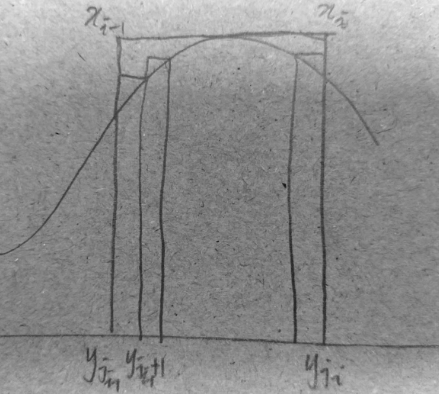
\includegraphics[width=0.5\linewidth]{images/RSintegral-partitions.png}
    \caption{Partitions}
\end{figure}

Continuing from
\[ \sup_{[x_{i-1},x_i]} f \ge \sup_{[y_{k-1},y_k]} f, \]
We then multiply by $\alpha(y_k)-\alpha(y_{k-1})$ on both sides and then take the sum from $k=j_{i-1}+1$ to $k=j_i$
:
The RHS corresponds to the (weighted) sum of the thin rectangles that you see in the above picture
:
The LHS is actually a telescoping sum, and the sum would be
\[ (\sup_{[x_{i-1},x_i]} f) \cdot [\alpha(y_{j_i})-\alpha(y_{j_{i-1}})] = (\sup_{[x_{i-1},x_i]} f) \cdot [\alpha(x_i)-\alpha(x_{i-1})] \]
Finally, we take the sum from $i=1$ to $i=n$ of the above inequality
LHS $\ge$ RHS (sorry I don't know of a better way to put it)
We then obtain $U(P,f,\alpha)\ge U(P^\prime,f,\alpha)$

(On the LHS we're collecting all the rectangles for the upper sum wrt $P$, but on the RHS we're collecting up collections of upper rectangles to obtain the entire collective of upper rectangles for the upper sum wrt $P^\prime$)
:
Lower sum is similar
:
Now, a lemma used to prove 6.5
Given any two partitions $P_1$ and $P_2$, we have
\[ L(P_1,f,\alpha)\le U(P_2,f,\alpha) \]
So a lower sum will always be no larger than any other upper sum
:
So this includes the cases where we have the most refined of $P_1$'s and $P_2$'s, with no information regarding the partition points whatsoever
To be honest, the result seems to be both intuitive and unclear at the same time

The key here is to use common refinements as a link for both sums
The idea is stated in the proof of 6.5 and I don't think I need to elaborate further

What's nice here is that now we have two completely independent partitions $P_1$ and $P_2$, so by fixing one partition, say $P_2$, and taking the 'limit' over the other (here we take the supremum over all possible $P_1$) we then obtain an inequality between a Darboux integral and a Darboux sum (here it's the lower integral and an upper sum)

Since the Darboux integral is just a number, we can then safely take the 'limit' over the other partition to obtain the inequality in 6.5
\end{proof}

\begin{proposition}
\[ \lowerint_a^bf\dd{\alpha}=\upperint_a^bf\dd{\alpha}. \]
\end{proposition}

\begin{proof}

\end{proof}

Now we move on to integrability conditions for $f$. The first one looks a lot like the $\epsilon-N$ or $\epsilon-\delta$ definition of limits:

\begin{theorem}
$f\in R_\alpha[a,b]$ if and only if for each $\epsilon>0$, there exists some partition $P$ such that
\[ U(f,\alpha;P)-L(f,\alpha;P)<\epsilon. \]
\end{theorem}
%%%%%%%%%%%%%%%%%%%%

\begin{proof} \

($\implies$) Assume $f\in R_\alpha[a,b]$. By definition,
\[ \inf_PU(f,\alpha;P)=\int_a^bf\dd{\alpha}=\sup_PL(f,\alpha;P). \]
For every $\epsilon>0$, 

($\impliedby$) 
\end{proof}



%%%%%%%%%%%%%%%%%%%%%%%%%
% Darboux sums, Darboux integrals

\begin{example}[Dirichlet function]
The Dirichlet function is given by
\[ f(x)=\begin{cases}
1 & x\in\QQ \\
0 & x\notin\QQ
\end{cases} \]
We try to calculate the two on the interval $[0,1]$.

The Dirichlet function is pathological because for each subinterval $[x_{i-1},x_i]$, the supremum is always $1$ and the infimum is always $0$.

So no matter what partition we use, $U(f,P)$ is always $1$ whereas $L(f,P)$ is always $0$. This means that $U(f)=1$ and $L(f)=0$, so there are two different values for ``the integral of $f$''.

This is like the case where we try to find the limit of the Dirichlet function where $x$ is approaching any given real number $r$, there exists two sequences approaching $r$ whose image approaches two different values.
\end{example}

Now, a very important and fun case about the more general RS-integral, which we'll discuss next week (do try the exercise yourself first)

\begin{exercise}
The Heaviside step function $H$ is a real-valued function defined by the following:
\[ H(x)=\begin{cases}
0 & x<0 \\
1 & x\ge0
\end{cases} \]
For the purpose of this question we assume the convention $\infty\cdot0=0$.
\begin{enumerate}[label=(\alph*)]
\item Let $f$ be a real-valued function over $\RR$. Show that $f\in\RR_H [a,b]$ iff $f$ is continuous at $0$, and find the RS-integral $\int_{-\infty}^\infty f\dd{H}$.
\item Suppose that the definition for $H$ is changed for $x=0$, say $H(0)=\frac{1}{2}$. Show that the above result still holds.
\item Examine the RS-integral of $f$ over $\RR\setminus\{0\}$ wrt $H$, where $f$ is a real-valued function over $\RR\setminus\{0\}$ such that $\lim_{x\to0}f(x)=\infty$ or $-\infty$.
\end{enumerate}
(You may read up on more information regarding the Heaviside function, and the (in)famous Dirac delta function)
\end{exercise}




Now we've been talking a lot about upper and lower sums because they're arguably the simplest way to define integrals, in the sense that there's not a whole lot of things that we could go wrong here
By considering only upper and lower bound, we're essentially picking the most conservative route possible

It would be nice if we could just pick like one random point within each interval and consequently calculate the Riemann(-Stieltjes) sums

This method, of course, fails to be well defined for pathological functions like the Dirichlet function
On the other hand, by using upper and lower sums, we could give a persuasive explanation as to why the Dirichlet function is not Riemann integrable

However, instead of throwing this idea away, there's actually a way for us to make this into a strict definition

When we were talking about the sequential definition for limits of functions, we noted that there are certain scenarios where the limit cannot exist because there may be two distinct sequences may give different limit
Based on this observation, we then gave a reasonable condition as follows:
"$\lim_{x\to a} f(x)$ exists and is equal to $L$ iff for all sequences $x_n$ converging but not containing a, $f(x_n)$ converges to $L$"

Well here, it's actually the same kind of scenario
Given any partition $P$, we consider the Riemann sum $\sum f(\xi_i)\Delta x_i$ where $\xi_i$ is any point where $x_{i-1}\le\xi_i\le x_i$

For the Dirichlet function over $[0,1]$, given any partition P (here we may assume that the partition points are distinct), we will always be able to specifically pick $\xi_i,\eta_i\in[x_{i-1},x_i]$ such that $\xi_i$ is rational but $\eta_i$ is irrational

Then $\sum f(\xi_i)\Delta x_i=1$ but $\sum f(\eta_i)\Delta x_i=0$

Now be very mindful that this alone cannot be evidence that f is non-integrable
The key is that this somehow occured for all partitions P, no matter how refined they are; for every single partition P, there exists two sets of 'representing points' $\xi_i,\eta_i$ such that the two Riemann sums are constantly far apart (1 and 0 in this case)

Let $\epsilon_0=1$, then this ultimately translates to the following:
The Dirichlet function cannot be Riemann integrable because
There exists some $\epsilon_0>0$, such that for any given partition $P$, there exists two sets of representing points $\xi_i,\eta_i$ such that their corresponding Riemann sums satisfy that
\[ |\sum f(\xi_i)\Delta x_i - \sum f(\eta_i)\Delta x_i|\ge\epsilon_0. \]

Now if we always pick the representatives such that $\xi_i>\eta_i$ then we can neglect the absolute value

So now, let's take the converse
A function $f$ is said to be RS-integrable if
For every $\epsilon>0$,
There exists a partition P, such that
For any two sets of representing points $\xi_i,\eta_i$,
Their corresponding Riemann sums satisfy that
\[ \sum[f(\xi_i)-f(\eta_i)]\Delta x_i<\epsilon \]
(The last one should be $\Delta \alpha_i$ for RS-integrals, not $\Delta x_i$)

Unfortunately this is still not quite the correct definition according to Apostol, but we're pretty close
The problem with this definition is that it is too weak if we're considering general $\alpha$ of bounded variation; if we were only talking about monotonically increasing $\alpha$ then this will actually be an equivalent definition

The official definition for the RS-integral wrt $\alpha$ of bounded variation is as follows:
\begin{definition}
For every $\epsilon>0$, there exists a partition $P$, such that
[For any refinement $P^\prime$ of P, and]
For any two sets of representing points $\xi_i,\eta_i$ [of $P^\prime$], their corresponding Riemann sums satisfy that
\[ \sum[f(\xi_i)-f(\eta_i)]\Delta x_i<\epsilon. \]
\end{definition}

Now this definition is what mathematicians would refer to as a 'Cauchy' definition, since it defines a notion by comparing a pair of arbitrary values that are similar to one another, and if they agree in some sense then we say that that something satisfies some property.

The integral is then obtained as follows: If $f$ were to satisfy the above Cauchy definition, then we may pick an arbitrary sequence of refinements
\[ P_1 \subset P_2 \subset P_3 \subset ...; \]
and for each partition we pick a set of representatives to obtain a sequence RS-sum
$I_1, I_2, I_3, ...$
:
This sequence will be a Cauchy sequence of real numbers, and so will converge to a specific value $I$ which we consider to be RS-integral of f
:
Now the reason why Apostol needed to strengthen the definition is that, otherwise this value $I$ may not be unique
:
So if you look at the statement you see in 6.7(b)(c), then they correspond to the Cauchy definition and the 'value-based' definition respectively
For monotonically increasing $\alpha$, it is much easier to discuss them using upper and lower sums
So your exercise today will be to read the statements and proofs in Theorem 6.7

\begin{theorem}
$f\in R_\alpha[a,b]$, $m\le f\le M$, and $\phi$ is uniformly continuous on $[m,M]$, then
\[ \phi\circ f\in R_\alpha[a,b]. \]
\end{theorem}

\begin{proof}
Choose $\epsilon>0$. Since $\phi$ is uniformly continuous on $[m,M]$, there exists $\delta>0$ such that $\delta<\epsilon$ and $|\phi(s)-\phi(t)|$
\end{proof}

\section{Properties of the Integral}
\begin{theorem} \
\begin{enumerate}[label=(\arabic*)]
\item If $f_1,f_2\in R_\alpha[a,b]$, then 
\[ f_1+f_2\in R_\alpha[a,b]; \]
$cf\in R_\alpha[a,b]$ for every $c\in\RR$, and
\[ \int_a^b(f_1+f_2)\dd{\alpha}=\int_a^bf_1\dd{\alpha}+\int_a^bf_2\dd{\alpha}, \]
\[ \int_a^b(cf)\dd{\alpha}=c\int_a^bf\dd{\alpha}. \]

\item If $f_1,f_2\in R_\alpha[a,b]$ and $f_1\le f_2$, then
\[ \int_a^bf_1\dd{\alpha}\le\int_a^bf_2\dd{\alpha}. \]

\item If $f\in R_\alpha[a,b]$ and $c\in[a,b]$, then $f\in R_\alpha[a,c]$ and $f\in R_\alpha[c,b]$, and
\[ \int_a^bf\dd{\alpha}=\int_a^c\dd{\alpha}+\int_c^b\dd{\alpha}. \]

\item If $f\in R_\alpha[a,b]$ and $|f|\le M$, then
\[ \absolute{\int_a^bf\dd{\alpha}}\le M\sqbrac{\alpha(b)-\alpha(a)}. \]

\item If $f\in R_{\alpha_1}[a,b]$ and $f\in R_{\alpha_2}[a,b]$, then $f\in R_{\alpha_1+\alpha_2}[a,b]$ and
\[ \int_a^bf\dd{(\alpha_1+\alpha_2)}=\int_a^bf\dd{\alpha_1}+\int_a^bf\dd{\alpha_2}; \]
if $f\in R_\alpha[a,b]$ and $c$ is a positive constant, then $f\in R_{c\alpha}[a,b]$ and
\[ \int_a^bf\dd{(c\alpha)}=c\int_a^bf\dd{\alpha}. \]

\item If $f\in R_\alpha[a,b]$ and $g\in R_\alpha[a,b]$, then $fg\in R_\alpha[a,b]$.
\end{enumerate}
\end{theorem}

\begin{proof} \
\begin{enumerate}[label=(\arabic*)]
\item If $f=f_1+f_2$ and $P$ is any partition of $[a,b]$, we have
\begin{align*}
L(f_1,\alpha;P)+L(f_2,\alpha;P)&\le L(f,\alpha;P)\\
&\le U(f,\alpha;P)\\
&\le U(f_1,\alpha;P)+U(f_2,\alpha;P).
\end{align*}

If $f_1\in R_\alpha[a,b]$ and $f_2\in R_\alpha[a,b]$, let $\epsilon>0$ be given. There are partitions $P_1$ and $P_2$ such that


\item 
\item 
\item 
\item 
\item 
\end{enumerate}
\end{proof}

\begin{theorem}[Triangle inequality]
$f\in R_\alpha[a,b]$, then $|f|\in R_\alpha[a,b]$,
\[ \absolute{\int_a^bf\dd{\alpha}}\le\int_a^b|f|\dd{\alpha}. \]
\end{theorem}

\begin{proof}

\end{proof}

6.14 6.15
Heaviside step function

6.16 corollary
for intinite sum, need $\sum c_n$ to converge
(23) comparison test

6.17 integration by substitution
\begin{theorem}
$\alpha$ increasing, $\alpha^\prime\in R[a,b]$, $f$ bounded on $[a,b]$, then
\[ f\in R_\alpha[a,b]\iff f\alpha^\prime\in R[a,b]. \]
\end{theorem}

6.19 change of variables

\section{Fundamental Theorem of Calculus}
6.20 6.21

\begin{theorem}

\end{theorem}

6.22 integration by parts

\chapter{Sequence and Series of Functions}
\section{Uniform Convergence}
\begin{definition}
Suppose $\{f_n\}$, $n=1,2,3,\dots$ is a sequence of functions defined on a set $E$, and suppose that the sequence of numbers $\{f_n(x)\}$ converges for every $x\in E$. We can then define a function $f$ by
\[ f(x)=\lim_{n\to\infty}f_n(x). \]
We say that $\{f_n\}$ \vocab{converges pointwise} to $f$ on $E$, denoted by $f_n\to f$.

Similarly, if $\sum f_n(x)$ converges for every $x\in E$, and if we define
\[ f(x)=\sum_{n=1}^\infty f_n(x) \]
the function $f$ is called the \vocab{sum of the series} $\sum f_n$.
\end{definition}
pointwise convergence

\begin{definition}
Assume $\{f_n\}$ is a sequence of functions defined over a set $X$ and $f$ is also a function defined over $X$. We say $\{f_n\}$ \vocab{uniformly converges} to $f$ over $X$, if for any $\epsilon>0$, there exists $N>0$ (which is independent of $x$) so that for any $x\in X$,
\[ |f_n(x)-f(x)|<\epsilon. \]
\end{definition}

\begin{notation}
We denote this uniform convergence over $X$ by $f_n\rightrightarrows f$.
\end{notation}

\section{Uniform Convergence and Continuity}

\section{Uniform Convergence and Integration}
\begin{theorem}
Assume $\{f_n\}$ is a sequence of functions defined over $[a,b]$ and each $f_n\in R_\alpha[a,b]$. If $f_n\to f$, then $f\in R_\alpha[a,b]$, and
\[ \lim_{n\to\infty}\int_a^bf_n\dd{\alpha}=\int_a^bf\dd{\alpha}. \]
\end{theorem}

\begin{proof}
Define
\end{proof}

\begin{corollary}
Assume $a_n\in R_\alpha[a,b]$ and
\[ f(x)\coloneqq\sum_{n=0}^\infty a_n(x) \]
converges uniformly. Then it follows
\[ \int_a^bf\dd{\alpha}=\sum_{n=0}^\infty a_n\dd{\alpha}. \]
\end{corollary}

\begin{proof}
Consider the sequence of partial sums 
\[ f_n(x)\coloneqq\sum_{k=0}^na_k(x), \quad n=0,1,\dots \]
It follows $f_n\in R_\alpha[a,b]$ and $f_n\rightrightarrows f$. Apply above theorem to $\{f_n\}$ and the conclusion follows.
\end{proof}

\section{Uniform Convergence and Differentiation}
\begin{theorem}
Assume $\{f_n\}$ is a sequence of functions defined over $[a,b]$ and differentiable. If $\{f_n^\prime\}$ uniformly converges on $[a,b]$ and $\{f_n\}$ converges at some point $x_0\in[a,b]$, then $\{f_n\}$ uniformly converges on $[a,b]$ to some function $f$. Moreover, $f$ is differentiable and
\[ f^\prime(x)=\lim_{n\to\infty}f_n^\prime(x) \]
for any $x\in[a,b]$.
\end{theorem}

\begin{proof}

\end{proof}

\section{Stone--Weierstrass Approximation Theorem}


\chapter{Some Special Functions}
\section{Power Series}
We derive some properties of functions represented by \vocab{power series}, i.e. functions of the form
\[ f(x)=\sum_{n=0}^\infty c_nx^n \]
or, more generally,
\[ f(x)=\sum_{n=0}^\infty c_n(x-a)^n. \]
These are called \vocab{analytic functions}.

If $f(x)$ converges for $|x-a|<R$, $f$ is said to be expanded in a power series about the point $x=a$. For convenience, we take $a=0$ without loss of generality. We call $R$ the \vocab{radius of convergence}.

\begin{theorem}
Suppose the series 
\[ \sum_{n=0}^\infty c_nx^n \]
converges for $x\in(-R,R)$. Then
\begin{enumerate}[label=(\arabic*)]
\item $\sum_{n=0}^\infty c_nx^n$ converges uniformly on the closed interval $[-R,R]$;
\item $f(x)$ is continuous and differentiable on $(-R,R)$, and 
\[ f^\prime(x)=\sum_{n=1}^\infty nc_nx^{n-1}. \]
\end{enumerate}
\end{theorem}

\begin{proof} \
\begin{enumerate}[label=(\roman*)]
\item 
\item 
\end{enumerate}
\end{proof}